\documentclass[11pt,a4paper]{article}
% Shared article style for handouts.
\usepackage[fontset=none]{ctex}
\usepackage{fontspec}
\setmainfont{DejaVu Serif}
\setsansfont{DejaVu Sans}
\setmonofont{DejaVu Sans Mono}
\setCJKmainfont{Noto Serif CJK SC}[BoldFont={Noto Serif CJK SC Bold}]
\setCJKsansfont{Noto Sans CJK SC}[BoldFont={Noto Sans CJK SC Bold}]
\setCJKmonofont{Noto Sans Mono CJK SC}

\usepackage[margin=1in]{geometry}
\usepackage{graphicx}
\usepackage{enumitem}
\usepackage{amsmath,amssymb}
\usepackage{booktabs,array}
\usepackage{xcolor}
\usepackage{listings}
\usepackage{tcolorbox}
\tcbuselibrary{breakable}
\usepackage{hyperref}

\definecolor{hcPrimary}{RGB}{20,72,110}
\definecolor{hcTipBG}{RGB}{239,246,252}
\definecolor{hcTipFrame}{RGB}{80,126,160}
\definecolor{hcWarnBG}{RGB}{253,244,238}
\definecolor{hcWarnFrame}{RGB}{183,84,52}
\definecolor{hcCodeBG}{RGB}{247,248,250}
\definecolor{hcCodeFrame}{RGB}{208,214,220}

\hypersetup{colorlinks=true,linkcolor=hcPrimary,urlcolor=hcPrimary,citecolor=hcPrimary}
\setlist{nosep}

\newtcolorbox{tipbox}{
  colback=hcTipBG,
  colframe=hcTipFrame,
  title=提示,
  fonttitle=\bfseries,
  boxrule=0.6pt,
  breakable
}

\newtcolorbox{warnbox}{
  colback=hcWarnBG,
  colframe=hcWarnFrame,
  title=警告,
  fonttitle=\bfseries,
  boxrule=0.6pt,
  breakable
}

\lstset{
  basicstyle=\ttfamily\footnotesize,
  backgroundcolor=\color{hcCodeBG},
  frame=single,
  rulecolor=\color{hcCodeFrame},
  numbers=left,
  numberstyle=\tiny,
  breaklines=true,
  showstringspaces=false,
  tabsize=2
}


\title{第一章：芯片、系统与产业全景}
\author{Digital Circuit Getting Started}
\date{\today}

\graphicspath{{figures/}}

\begin{document}
\maketitle

\section{本章导读}

这本书的第一章，不会上来就扔给你一堆术语，也不会让你去背公司名字。我们想先解决一个更根本的问题：后面要学的数字电路、RTL、验证、综合与实现，究竟在一张怎样的地图上。

很多人刚接触数字设计时，就直接扎进逻辑门、真值表和 Verilog 语法里。学着学着，心里总会冒出一些挥之不去的困惑：芯片到底是什么？那块黑色封装件和里面裸硅片是什么关系？为什么一台设备里不只有一颗芯片，而是主控、存储、电源、接口器件一整套在协同工作？为什么有的公司设计芯片，有的做工具，有的造晶圆？如果这些问题没有先理清楚，后面学到的知识很容易变成一堆彼此割裂的局部技巧——你知道每个模块怎么写，却拼不出一张完整的图景。

所以在进入整个课程之前，希望带领大家建立一张认知地图：首先是我们会从``为什么复杂系统必须依赖抽象''开始；然后把视角拉回真实世界，看看集成电路怎么就成了现代电子系统的主流范式，一颗裸片怎么变成能焊到板子上的器件，又怎么和电源、时钟、存储、接口一起构成一个能跑起来的系统；最后再延伸到芯片类型、设计流程、产业链分工，以及一个工程上很实用的思考习惯——3Y 三问法。

如果你是自学者，这张地图尤其重要。课堂里老师可以不断提醒你这一块以后会在哪里用到，但自学时，材料往往是一章接一章静静摆在你面前。没有地图，人就容易迷路；有了地图，即使暂时还走得慢，也知道自己正朝哪个方向前进。

这章读完后，你不会立刻学会设计芯片，但你会知道后面每一章在整张地图上的位置。这样再遇到新概念时，心里会有一个坐标，而不是碎片。

\section{Learning Objectives}

读完这一章，你会：

\begin{itemize}
  \item 理解为什么数字系统设计中，抽象和分层不是装饰性的说法，而是工程推进过程中自然长出来的组织方式。
  \item 搞清楚数字抽象到底在``抽象''什么，以及它在什么前提下会失效。
  \item 明白从分立电路到 IC 再到 SoC，集成化是怎么一步步成为现代电子工程的主流范式的。
  \item 分得清 \texttt{die}、\texttt{package}、\texttt{chip}、板级器件和系统这几个层次，不再混着叫``芯片''。
  \item 知道封装到底在解决什么问题——不只是``套个壳''那么简单。
  \item 看懂一颗芯片在板子上是怎么和电源、时钟、复位、存储、接口一起协同工作的。
  \item 对常见芯片类型、设计流程和产业链分工建立第一层整体认知，至少能说出几个典型公司大概在做什么。
  \item 理解工具链、文档、参考设计和生态为什么也会影响芯片竞争力，但不会把它们误解为产业链的全部。
  \item 掌握一个实用的思考习惯——3Y 三问法——用来分析任何芯片或模块。
\end{itemize}

\section{为什么复杂系统必须依赖抽象}

\subsection{从复杂度膨胀开始}

想象你面对的不是课堂上的几个逻辑门，而是一颗现代智能手机的主处理器（SoC）。它内部集成了 CPU 多核集群、GPU、AI 引擎、图像信号处理器、显示控制器、存储器接口、无线通信基带和数十种外设控制器。晶体管数量以百亿计。

\begin{figure}[h]
  \centering
  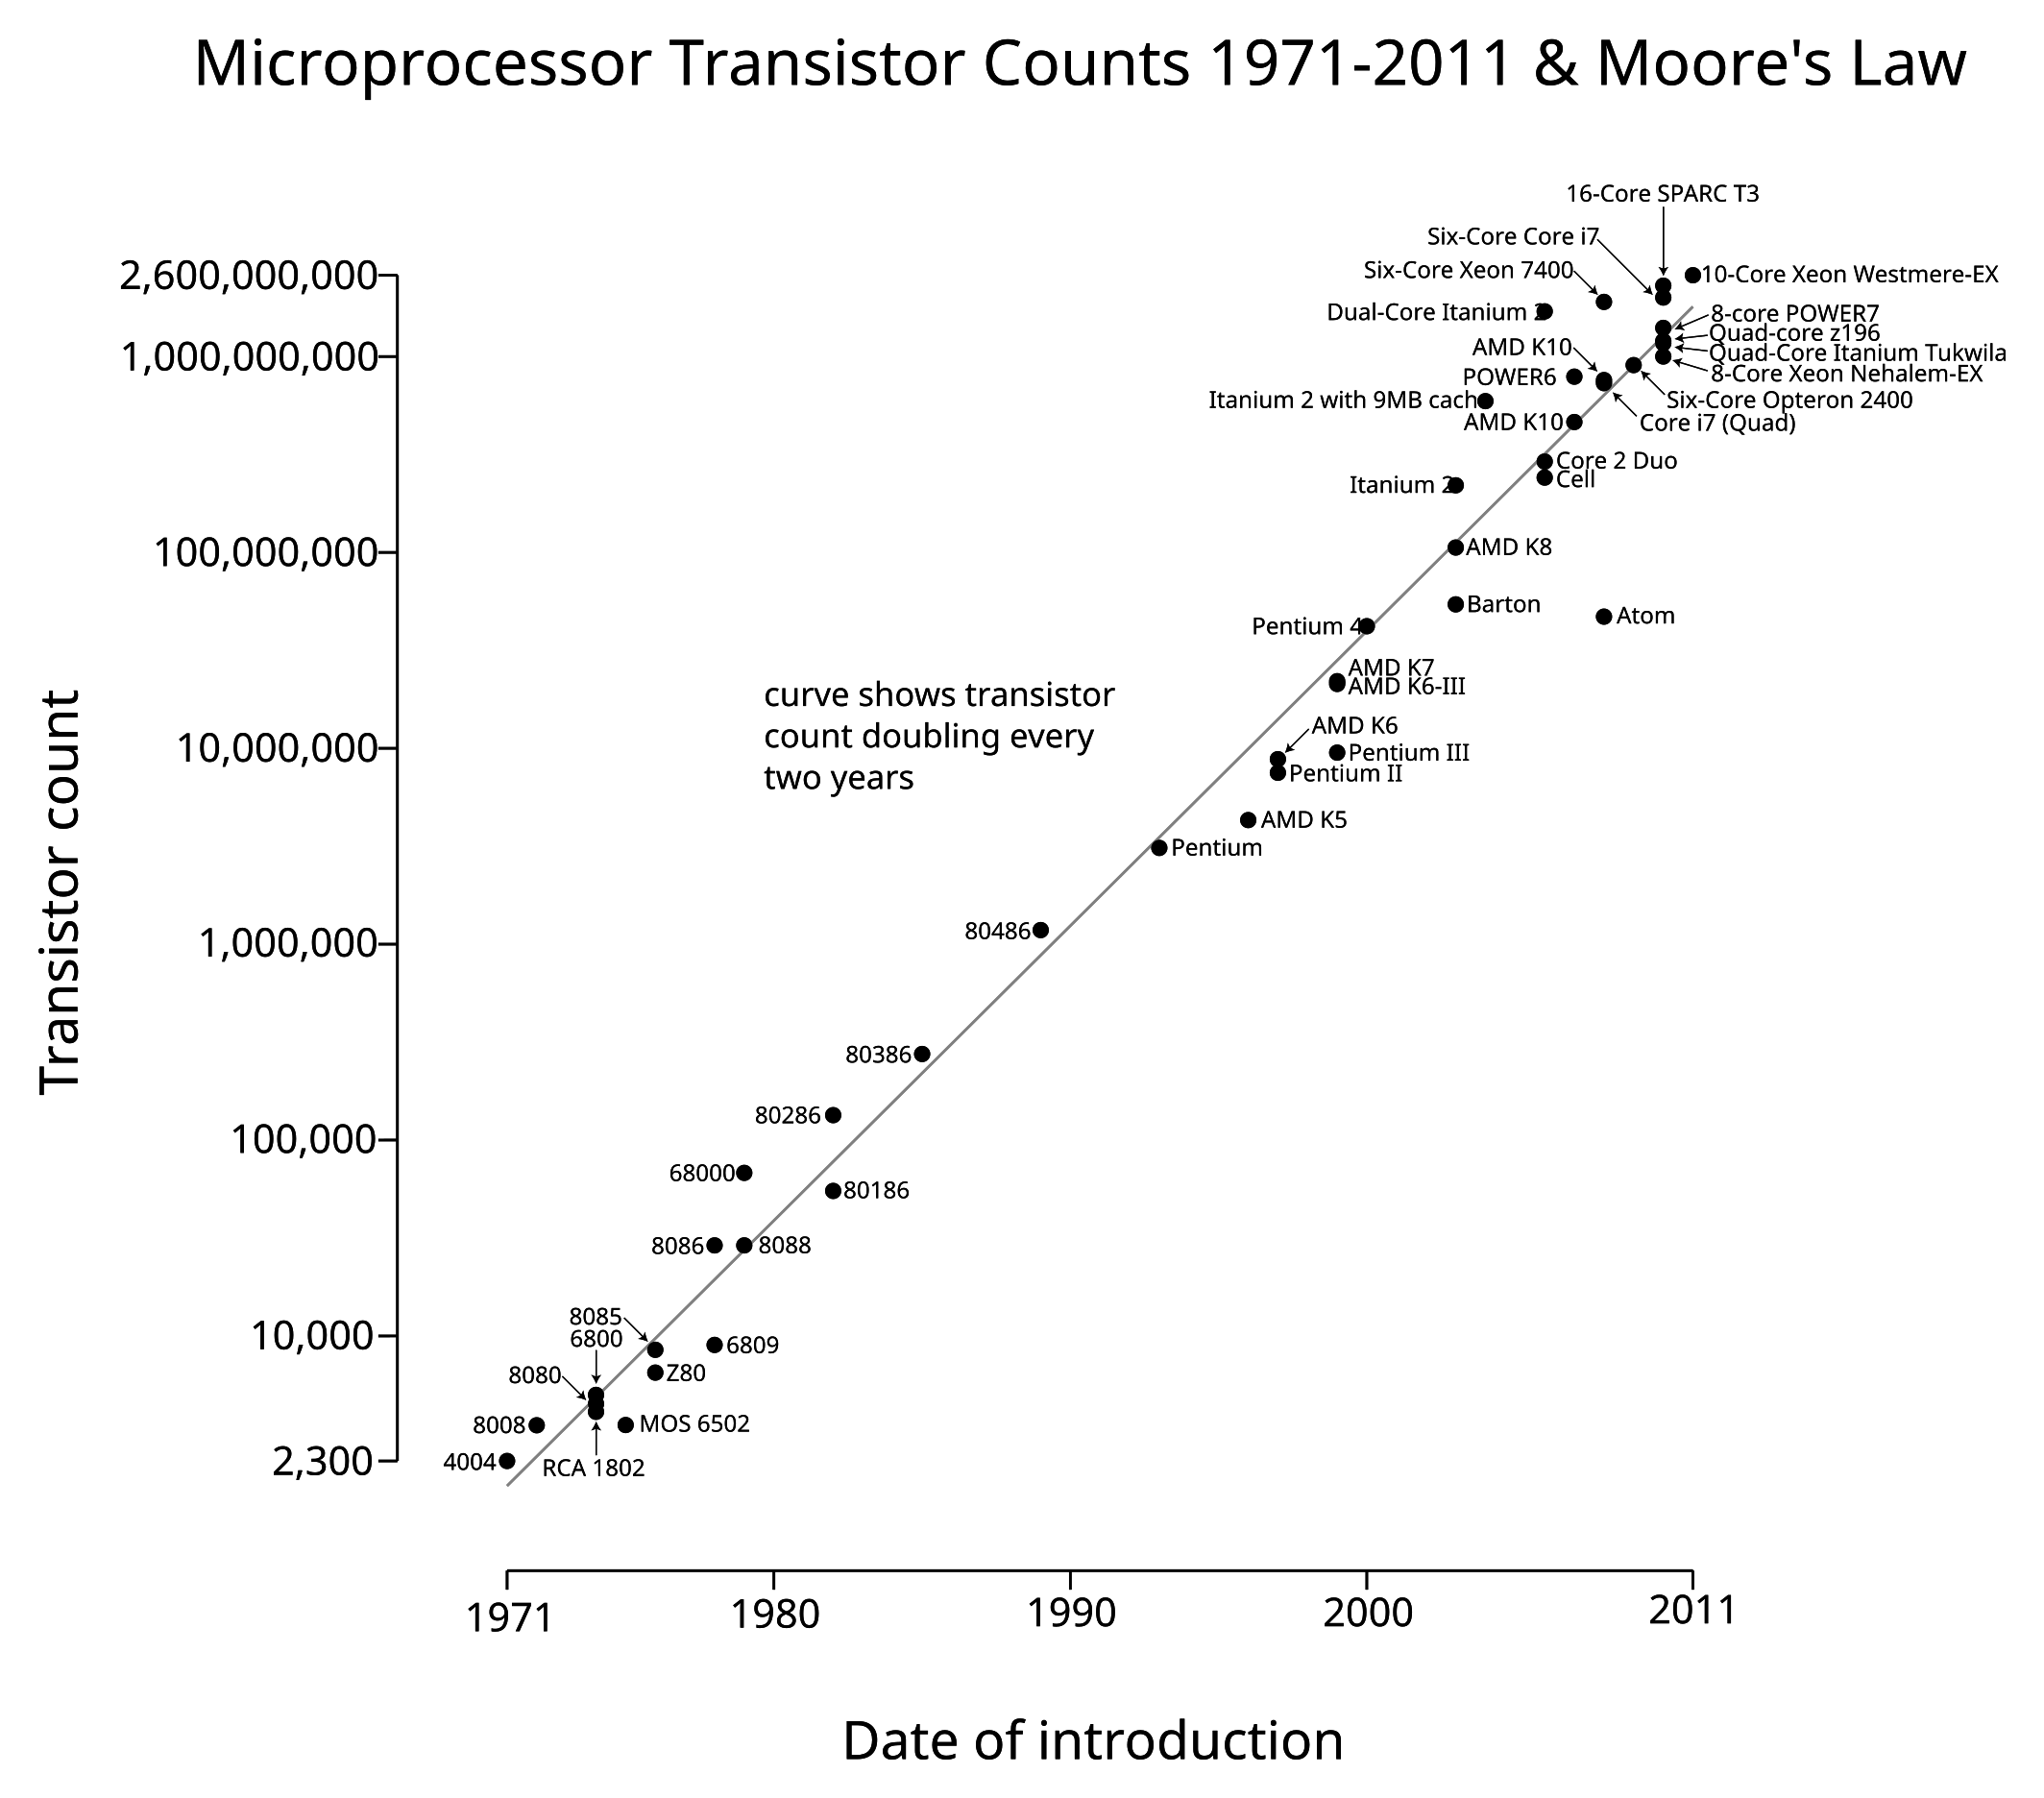
\includegraphics[width=0.74\linewidth]{moore.png}
  \caption{晶体管规模持续增长，意味着设计复杂度必须依赖抽象来管理。}
\end{figure}

复杂度一旦上升到这个量级，设计工作的重心就会自然转移。问题不再只是功能``能不能做出来''，而是这个功能能不能被组织成``清楚、稳定、能验证、能修改的结构''。

抽象正是为了回答这个问题而存在的。它服务于一个务实的工程目标：让复杂系统真正可操作。

换句话说，抽象不是把难题``消灭''掉，而是把它们重新安排。哪些问题应该现在处理，哪些问题应该留到后面处理，哪些问题应该通过接口交给别人处理，哪些问题必须用验证来兜底，这些都属于抽象设计的一部分。一个成熟的工程系统，往往不是因为它没有复杂性，而是因为复杂性被安放在了合适的位置。

\begin{tipbox}
这里可以先建立一个直觉：系统里每多几个能存 0 或 1 的存储位，所有可能组合就会指数增长。10 个存储位有 $2^{10}=1024$ 种组合，32 个就超过 40 亿。后面我们会把这种现象正式叫做``状态空间爆炸''——它解释了为什么复杂芯片不能靠穷举来设计。
\end{tipbox}

\subsection{抽象如何帮助设计}

抽象的核心思想并不复杂：在某一层只关心该层真正需要面对的问题，把更底层的细节暂时收起来。

以 RTL 设计为例。当你在 Verilog 里描述``两个寄存器之间的加法''时，你关注的是数据宽度、时钟边沿和运算符号。你不会在每一行代码里重新琢磨底层 MOS 管怎么导通，也不会去算每个反相器的传播延迟。这些物理细节当然重要——它们决定了芯片最终能不能跑在目标频率上——但它们属于时序分析和物理设计阶段的问题，不需要在功能建模阶段搅在一起。

反过来，当器件工程师分析标准单元库的驱动能力和漏电流时，同样不会把模块端口列表和总线协议搬出来解释电压摆幅。这不是在偷懒，而是把复杂性安置到当前最合适的层次上。

抽象不会让复杂性凭空消失。一旦接口、时序、电平或功耗边界被突破，底层细节就会重新回来主导结果。所以抽象不是对现实的否认，而是一种有控制的延期处理——现在先不处理，但要知道在什么条件下它一定会``回来''。

这也是为什么大规模芯片设计天然适合团队协作。有人位于架构层思考系统目标，有人站在 RTL 层组织模块行为，有人盯着验证，有人则关注着时序和物理实现。每个人不需要同时抱住全部复杂性，但整个团队必须通过清楚的接口和一致的抽象层次把工作接起来。没有抽象，团队只会互相干扰；有了抽象，团队才有可能并行推进。

在数字系统中，常见的抽象层次自顶向下至少包括五层：

\begin{itemize}
  \item \textbf{System / 系统层}：性能、功耗、带宽、软件配合和整机角色，例如 SoC、PCB 系统、设备整机等。
  \item \textbf{Module / 模块层}：端口、协议、功能边界和模块间协作，例如总线、DMA、Cache 等子系统在此层组织。
  \item \textbf{Gate / 逻辑门层}：布尔功能、门级连接和基本逻辑结构。
  \item \textbf{Circuit / 电路层}：门级单元的驱动能力、扇出、转换时间、功耗，主要关注 CMOS 门电路的晶体管级实现。
  \item \textbf{Device / 器件层}：MOS 管导通条件、电压、电流、延迟、噪声和物理行为。
\end{itemize}

\begin{center}
\setlength{\tabcolsep}{14pt}
\renewcommand{\arraystretch}{1.4}
\begin{tabular}{@{}c c@{}}
\raisebox{-0.5\height}{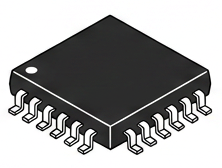
\includegraphics[width=1.6cm]{system.png}}  & \raisebox{-0.5\height}{\textbf{\large System / 系统层}}  \\
                                                                    & {\Large $\Uparrow$}                                      \\
\raisebox{-0.5\height}{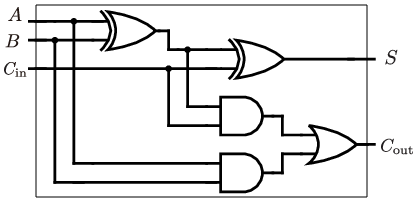
\includegraphics[width=1.6cm]{module.png}}  & \raisebox{-0.5\height}{\textbf{\large Module / 模块层}}  \\
                                                                    & {\Large $\Uparrow$}                                      \\
\raisebox{-0.5\height}{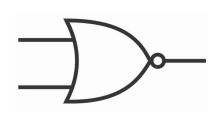
\includegraphics[width=1.6cm]{gate.png}}    & \raisebox{-0.5\height}{\textbf{\large Gate / 逻辑门层}}  \\
                                                                    & {\Large $\Uparrow$}                                      \\
\raisebox{-0.5\height}{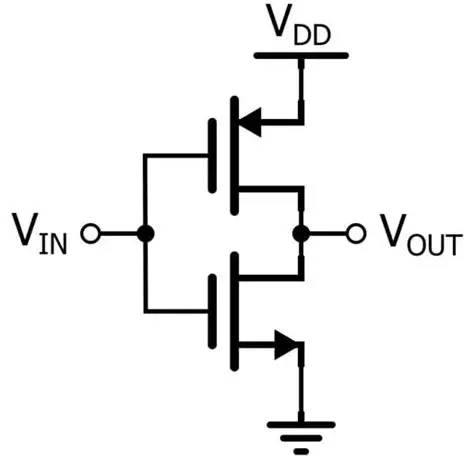
\includegraphics[width=1.6cm]{circuit.png}} & \raisebox{-0.5\height}{\textbf{\large Circuit / 电路层}} \\
                                                                    & {\Large $\Uparrow$}                                      \\
\raisebox{-0.5\height}{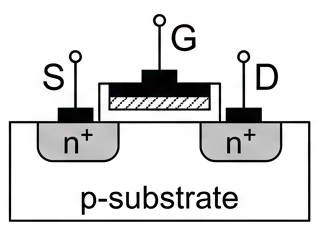
\includegraphics[width=1.6cm]{nmos.png}}    & \raisebox{-0.5\height}{\textbf{\large Device / 器件层}}
\end{tabular}
\end{center}

抽象层次可以类比为搭积木。如果每次搭一块新的积木，都要先把底层所有积木的分子结构计算一遍，那没有人能搭出一座城堡。抽象的作用，就是允许你信任这块积木在上一层的约定下是可用的，然后把精力集中在当前层的组合逻辑上。当然，这份信任不是无条件的，它要建立在接口、时序和电平都满足约定的前提上。

\subsection{数字抽象到底在抽象什么}

现实世界本质上是模拟的。电路中的信号是连续变化的电压和电流，器件会延迟，温度会影响它们的行为，工艺有偏差，噪声无处不在。如果始终停留在纯模拟视角来处理所有问题，工作量很快就会超出人力范围——别说设计一颗复杂芯片，哪怕只是组织一个稍大一点的数字模块，也会让人陷入连续信号的海洋里找不到岸。

数字抽象的做法，就是把一部分连续世界组织成离散的逻辑世界。具体来说：

\begin{itemize}
  \item 某个电压范围被定义为逻辑 0，另一个电压范围被定义为逻辑 1。
  \item 两个逻辑值之间的模糊区域被禁止，系统需要尽量保证信号不会长期停留在那里。
  \item 状态只在时钟边沿更新，组合逻辑在两个寄存器之间完成计算。
  \item 设计者关注的是结果能否在下一个时钟沿之前``准备好''，而不是每个晶体管的连续轨迹。
\end{itemize}

这样一来，设计者就能用精准（无歧义）的逻辑语言精准刻画系统。但数字抽象不是无条件成立的。它至少依赖三个前提：

\begin{itemize}
  \item 电平要足够可靠，不能让逻辑 0 和逻辑 1 混成模糊状态。
  \item 时序要成立，寄存器之间的数据要在正确的时钟沿之前稳定到达。
  \item 接口边界要明确，否则不同模块会在语义上互相冲突。
\end{itemize}

所以后面遇到的建立时间（setup time）、保持时间（hold time）、时钟偏斜（clock skew）、亚稳态（metastability）、接口协议，看似是各自独立的技术术语，实际上它们有一个共同任务：保护这层数字抽象不失效。下次再遇到这些概念时，不妨问自己一句：这个约束，是在保护哪一层的抽象不被突破？

本章在这里先把``数字抽象为什么成立、又为什么会失效''的骨架立住。到第三章再回头看这些词时，你会发现它们已经不只是词，而是在守护同一套秩序。

\begin{warnbox}
数字抽象不是天然成立的。它是一层人工构建的逻辑秩序，依赖物理世界的承诺来维持。当电压不够、时序不够或接口定义不清时，这层秩序就会崩塌。
\end{warnbox}

\section{为什么集成化成为现代电子的主导范式}

前面我们一直在谈方法论，现在把视角拉回工程现实。抽象之所以重要，不只是因为``系统很复杂''，还因为现代电子系统的默认起点已经不是分立器件，而是集成电路。如果把这条历史线按层级展开，可以看到一个逐级递增的过程：先有工艺级集成，再有功能单元级集成，随后发展出 IP 级集成，最后走向系统级集成。每上升一层，复杂性都会被搬运到一个更稳定、更可复制的边界上。

\subsection{工艺级集成：从 Kilby 和 Noyce 到平面工艺}

1958 年，Jack Kilby 在德州仪器（Texas Instruments）用一块锗片制成了世界上第一块集成电路。几个月后，Robert Noyce 在仙童半导体（Fairchild Semiconductor）独立发明了基于硅平面工艺的集成电路。两人后来共享了诺贝尔物理学奖，但他们的发明路径并不相同。

\begin{figure}[h]
  \centering
  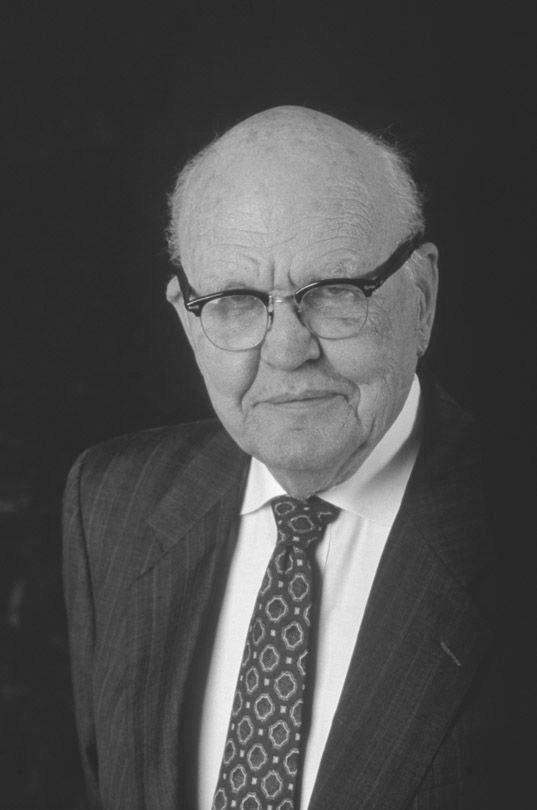
\includegraphics[width=0.38\linewidth]{kilby.jpg}
  \hspace{0.3cm}
  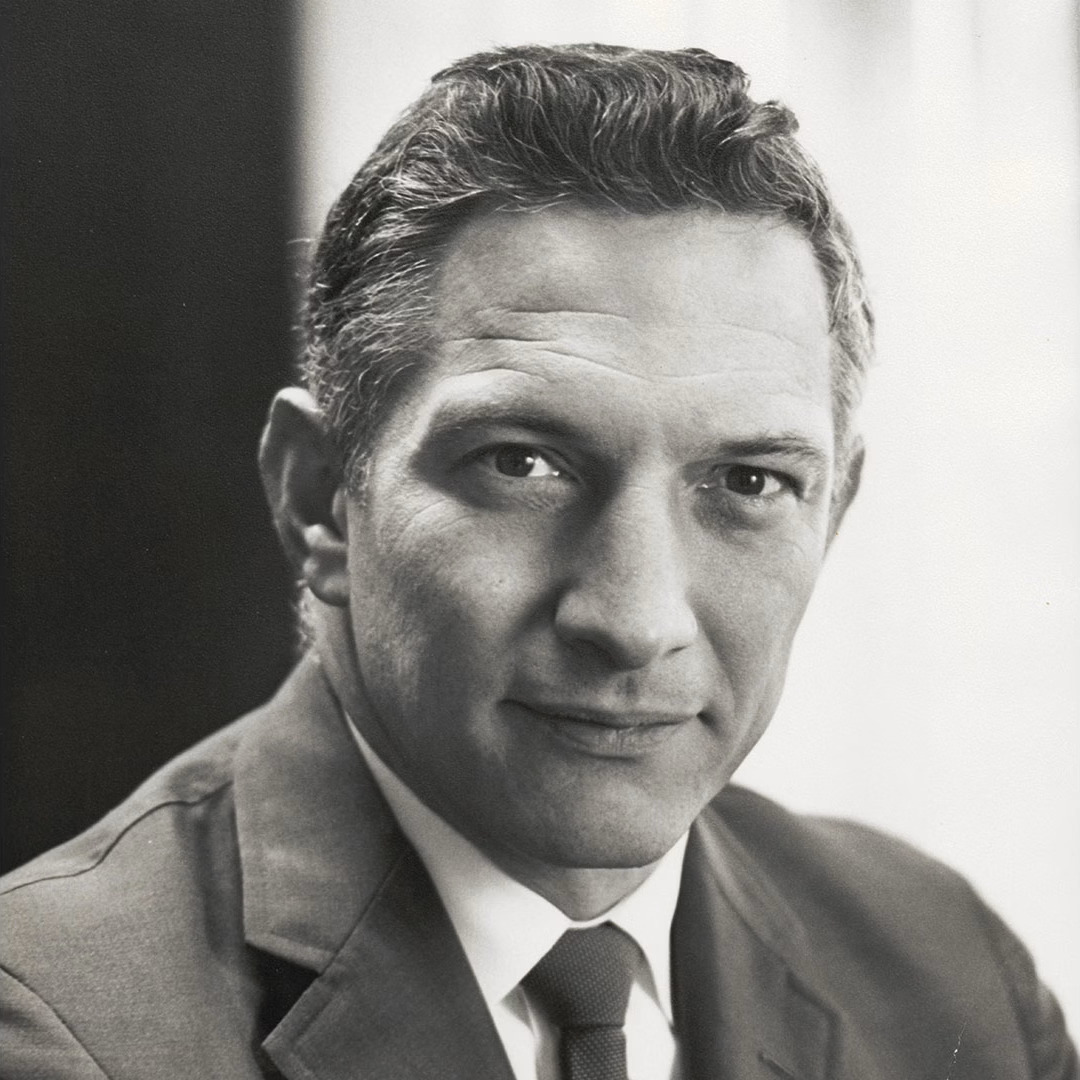
\includegraphics[width=0.40\linewidth]{noyce.jpg}
  \caption{Jack Kilby（左）在 TI 发明第一块锗基集成电路；Robert Noyce（右）在 Fairchild 发明硅平面工艺 IC。两人的工作共同开启了集成电路时代。}
\end{figure}

Kilby 用的是锗材料，Noyce 则用的是硅材料；Kilby 的方法更接近实验性验证，而 Noyce 的平面工艺更适合大规模生产。这个差异至关重要：集成电路的诞生不是单一闪光时刻，而是多条技术路线在竞争中的收敛。后来整个半导体产业建立在硅基之上，核心原因并不是硅听起来更``先进''，而是硅更容易和氧形成稳定的绝缘层，能把器件保护、图形定义、互连制造放进同一套平面工艺里；这样一来，光刻出来的结构也更容易被一批批重复复制，良率、成本和规模化才真正变得可控。

这段历史对今天的你意味着什么？意味着我们今天谈芯片，不是在谈某个孤立的``高科技零件''，而是在谈一种已经能够被稳定制造、重复复制的工程对象。也正因为制造端先被组织起来，后面才会依次长出标准单元、设计复用、EDA 工具链和更细的产业分工。所以，在第二章工具篇，我们将会接着这一层往下走：当制造已经成为可重复、可协作的工业流程时，设计也必然演化出对应的工程方法。

\subsection{单元级集成：从分立电路到标准芯片}

集成电路革命不只发生在数字领域，而且它之所以能扩展到模拟领域，前提正是集成电路制造本身先变得更成熟、更稳定、更可复制。1960 年代，Robert Widlar 在模拟 IC 设计上的工作就说明：当平面工艺已经能较可靠地批量制造器件与互连后，模拟电路也会被集成化重塑。他设计的 \textmu A702、\textmu A709，以及后来沿着同一路线走向普及的 \textmu A741，意味着原本需要大量分立晶体管和电阻拼出来的运放，可以被压缩进一颗标准化芯片中。

\begin{figure}[h]
  \centering
  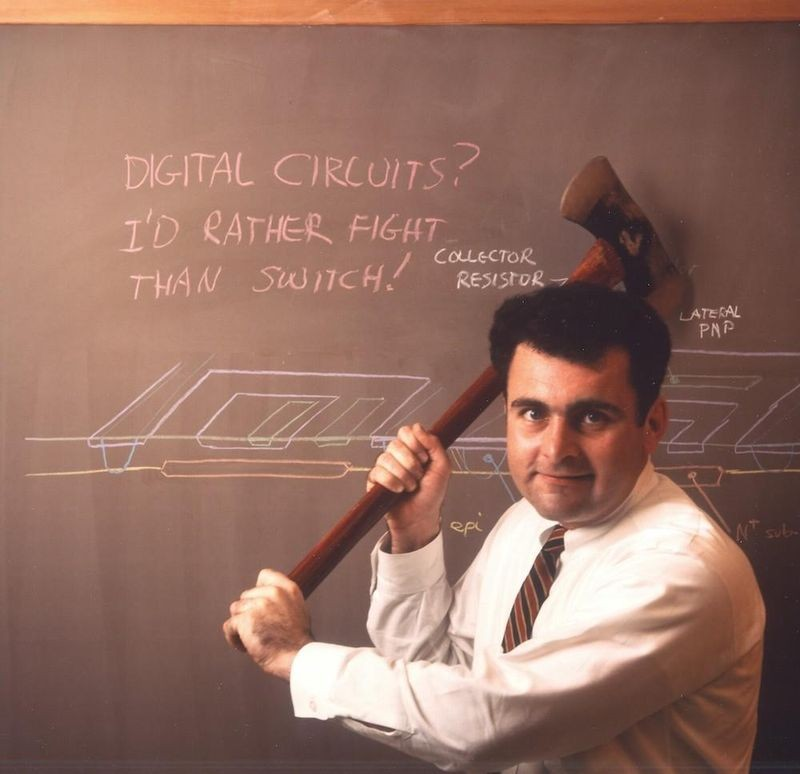
\includegraphics[width=0.38\linewidth]{widlar.jpg}
  \hspace{0.3cm}
  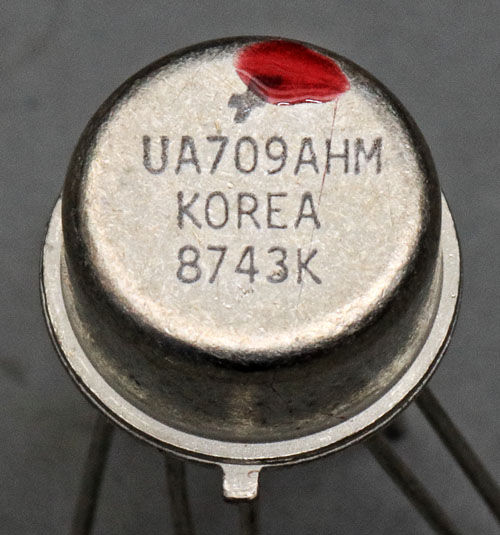
\includegraphics[width=0.28\linewidth]{ua709.jpg}
  \caption{Robert Widlar（左）与他设计的 \textmu A709 单片运放（右）。它的意义不只是一个产品成功，而是说明模拟电路也进入了集成化时代。}
\end{figure}

单元级集成化带来的关键变化在于：不再只是把更多晶体管放到同一块硅上，而是开始把运放、ADC、PMIC、驱动器这类功能单元做成标准芯片，供后续系统设计直接调用。

初学阶段尤其需要警惕一种错觉：数字世界代表现代工程，模拟领域还停留在分立器件时代。事实比二分法暗示的图景复杂得多。模拟、数字、混合信号、功率路径并不是彼此隔绝的几个宇宙，它们经常在同一个产品里相遇，也经常在同一颗芯片或同一封装里彼此配合。

\subsection{IP 级集成：从功能单元到设计积木}

当单元级集成稳定下来之后，设计活动本身也开始集成化。SoC 方法学的核心是 \textbf{IP 复用}：设计公司不必从零开发每个子系统，而是购买或授权标准化的 IP 模块，例如处理器核、接口控制器、模拟模块和存储控制器等。这些 IP 经过预先验证，可以带着清晰的接口和约束被直接集成到新的芯片设计中，缩短开发周期并降低风险。

IP 级集成带来的变化之所以重要，是因为它意味着工程师越来越少从晶体管甚至门级重新开始，而是越来越多在组织模块边界、接口契约、验证流程和工具链。标准接口、EDA 工具和团队分工，都是 IP 级集成继续扩大的必要条件。

\subsection{系统级集成：从 IC 到 SoC}

再往上一层，原本分散在板级系统上的大量功能开始被压进单颗芯片。这种范式转移在今天已经无处不在。一颗现代手机 SoC 在指甲盖大小的硅片上集成了 CPU、GPU、NPU、ISP、基带、存储控制器和数十种接口；一颗现代模拟或混合信号芯片内部，也往往同时包含模拟前端、数字校准逻辑、接口状态机，甚至与功率路径相关的器件结构。

\begin{figure}[h]
  \centering
  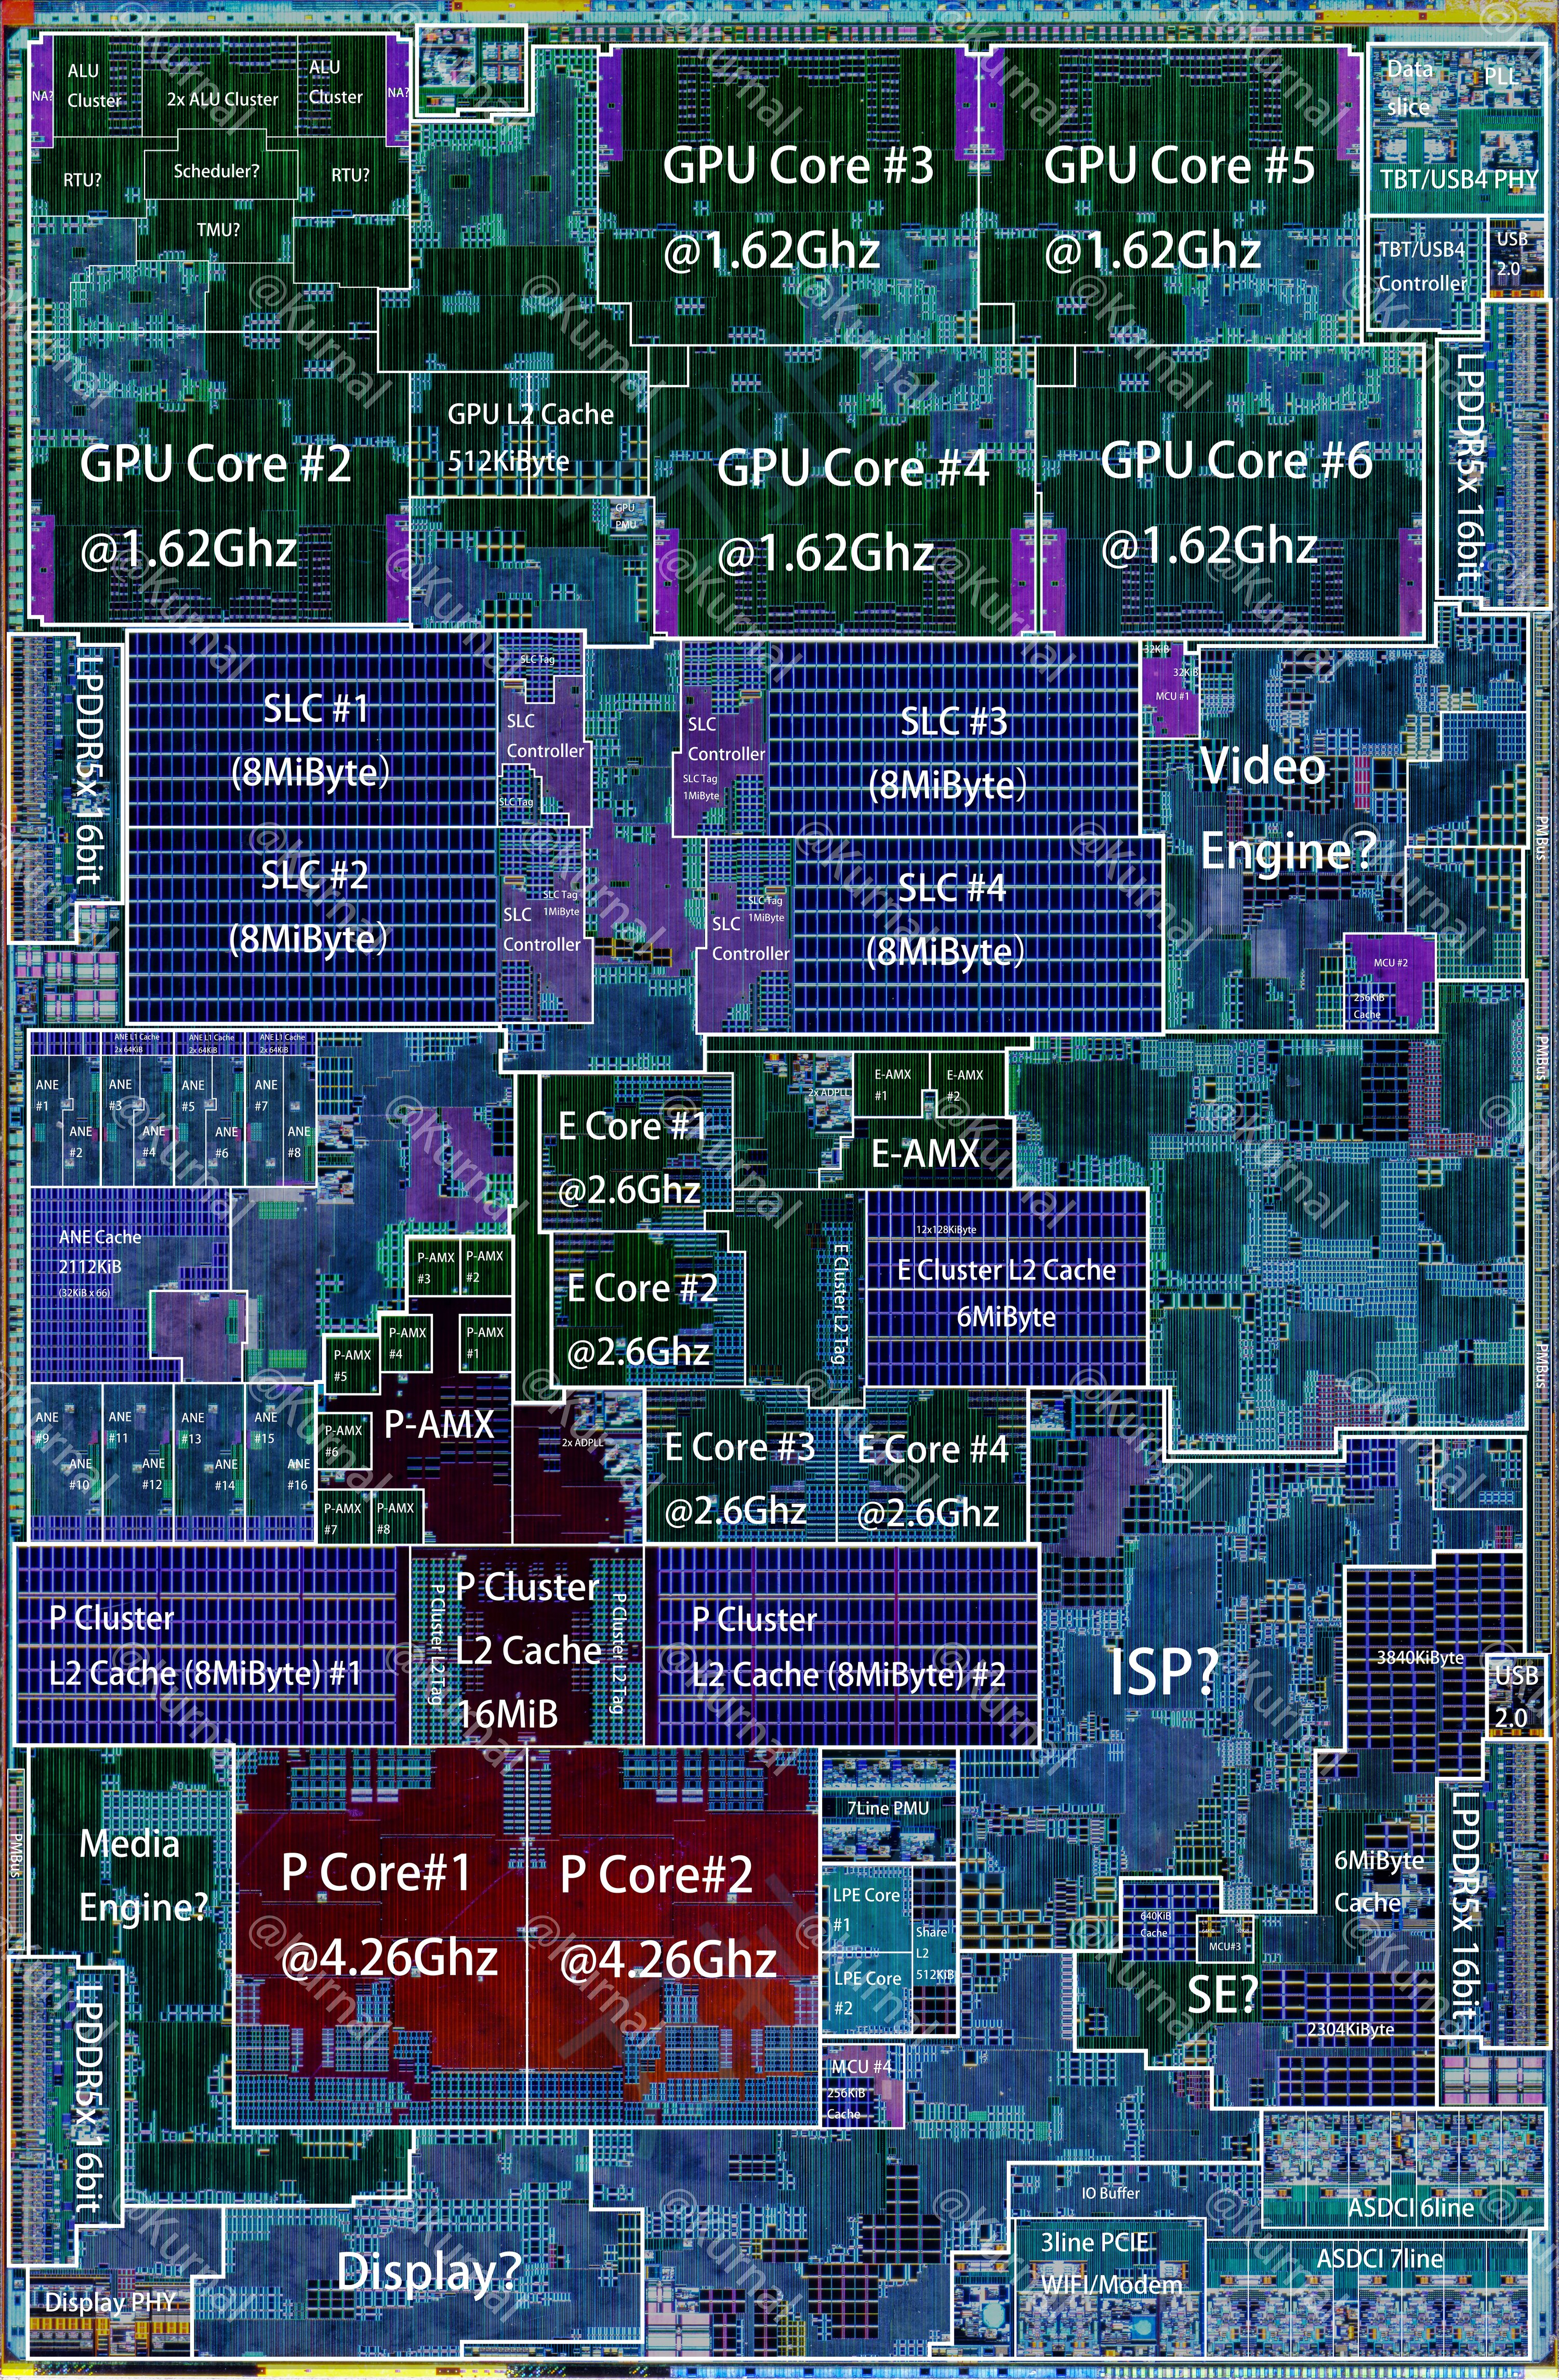
\includegraphics[width=0.48\linewidth]{a19p-layout.jpg}
  \hspace{0.2cm}
  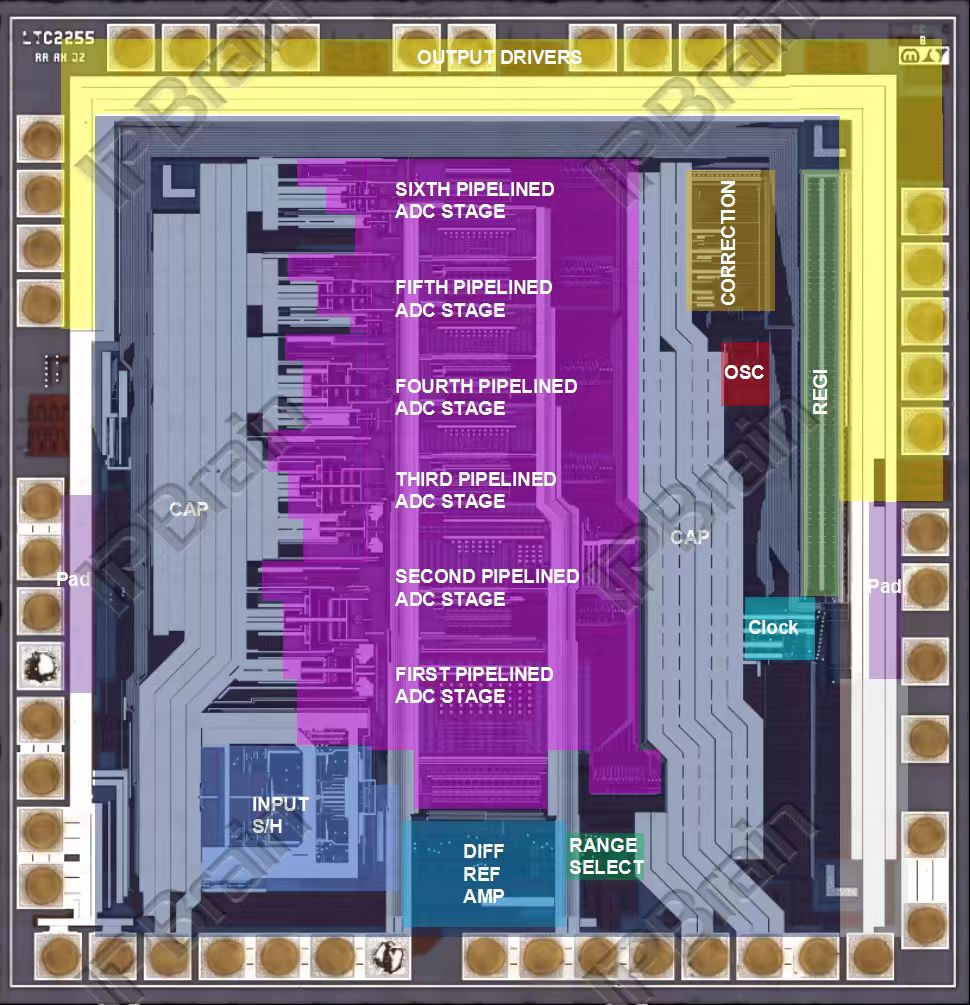
\includegraphics[width=0.44\linewidth]{adc_layout.jpg}
  \caption{现代芯片的高度集成：左图展示数字 SoC 的复杂度，右图展示模拟/混合信号芯片的集成度。两者都包含了相当数量的功能单元模块。}
\end{figure}

现代芯片设计也因此从``搭电路''进一步转向``搭系统''。对于那些直接销售芯片的公司，这种系统级集成甚至会继续向外延伸成``一站式方案''：参考设计、评估板、原理图、BOM 清单，甚至在线设计工具（如 TI 的 WEBENCH、ADI 的 LTpowerCAD）。这意味着工程师越来越多是在做选型、参数配置、系统整合和边界权衡，而不是从分立器件层面重新搭起整套功能。

\begin{tipbox}
历史线在本章中的作用，不是让你背年份，而是帮你形成一个判断：今天电子工程的默认起点是层层递进形成的集成范式，而不是分立范式。
\end{tipbox}

\section{从裸片到系统：我们到底在讨论什么对象}

\subsection{五个最容易混淆的词}

``芯片''这个词在日常生活中用得很宽。看到硅片叫芯片，看到封装件也叫芯片，看到板上的主控器件还是叫芯片。日常交流里这样叫问题不大，但一旦进入学习和分析系统，最好把几个对象区分开来。用错对象层次，就像把一栋建筑的``砖块''、``承重墙''、``房间''和``整栋楼''混为一谈——在这种混淆下，结构分析就无从谈起。

\begin{center}
\begin{tabular}{p{0.16\linewidth} p{0.76\linewidth}}
\toprule
术语 & 含义 \\
\midrule
\texttt{die} & 制造完成但尚未封装的裸片，真正承载晶体管和互连的硅片本体。 \\
\texttt{package} & 为裸片提供机械保护、电连接、散热路径和装配形态的封装结构。 \\
\texttt{chip} & 工程语境中通常指已经封装完成、可测试、可焊接、可装配的器件。 \\
\texttt{board} & 多个器件焊接在 PCB 上形成的板级系统，包含连线、电源网络和接口连接器。 \\
\texttt{system} & 由板卡、软件、供电、外设、通信链路等共同构成的完整工作整体。 \\
\bottomrule
\end{tabular}
\end{center}

\subsection{为什么要先分清这些对象}

后续几乎所有讨论都建立在对象层次之上。如果你在和同学聊沟道长度、漏电流或工艺层叠，你们聊的对象更接近 \texttt{die}；如果在讨论引脚怎么引出、焊球怎么散热、器件怎么装配，那话题已经进入了 \texttt{package}；如果在分析芯片和存储器、PMIC、时钟源之间怎么配合，那讨论的是 \texttt{board} 或 \texttt{system}。层次不同，关注的工程问题就完全不同。

一个简单的现实对应是：打开一台笔记本电脑的底盖，那些黑色方块是 \texttt{chip}；下面的绿色大板是 \texttt{board}；每个黑色方块内部那片硅才是 \texttt{die}；整个笔记本再加上操作系统和外设才构成 \texttt{system}。

\begin{figure}[h]
  \centering
  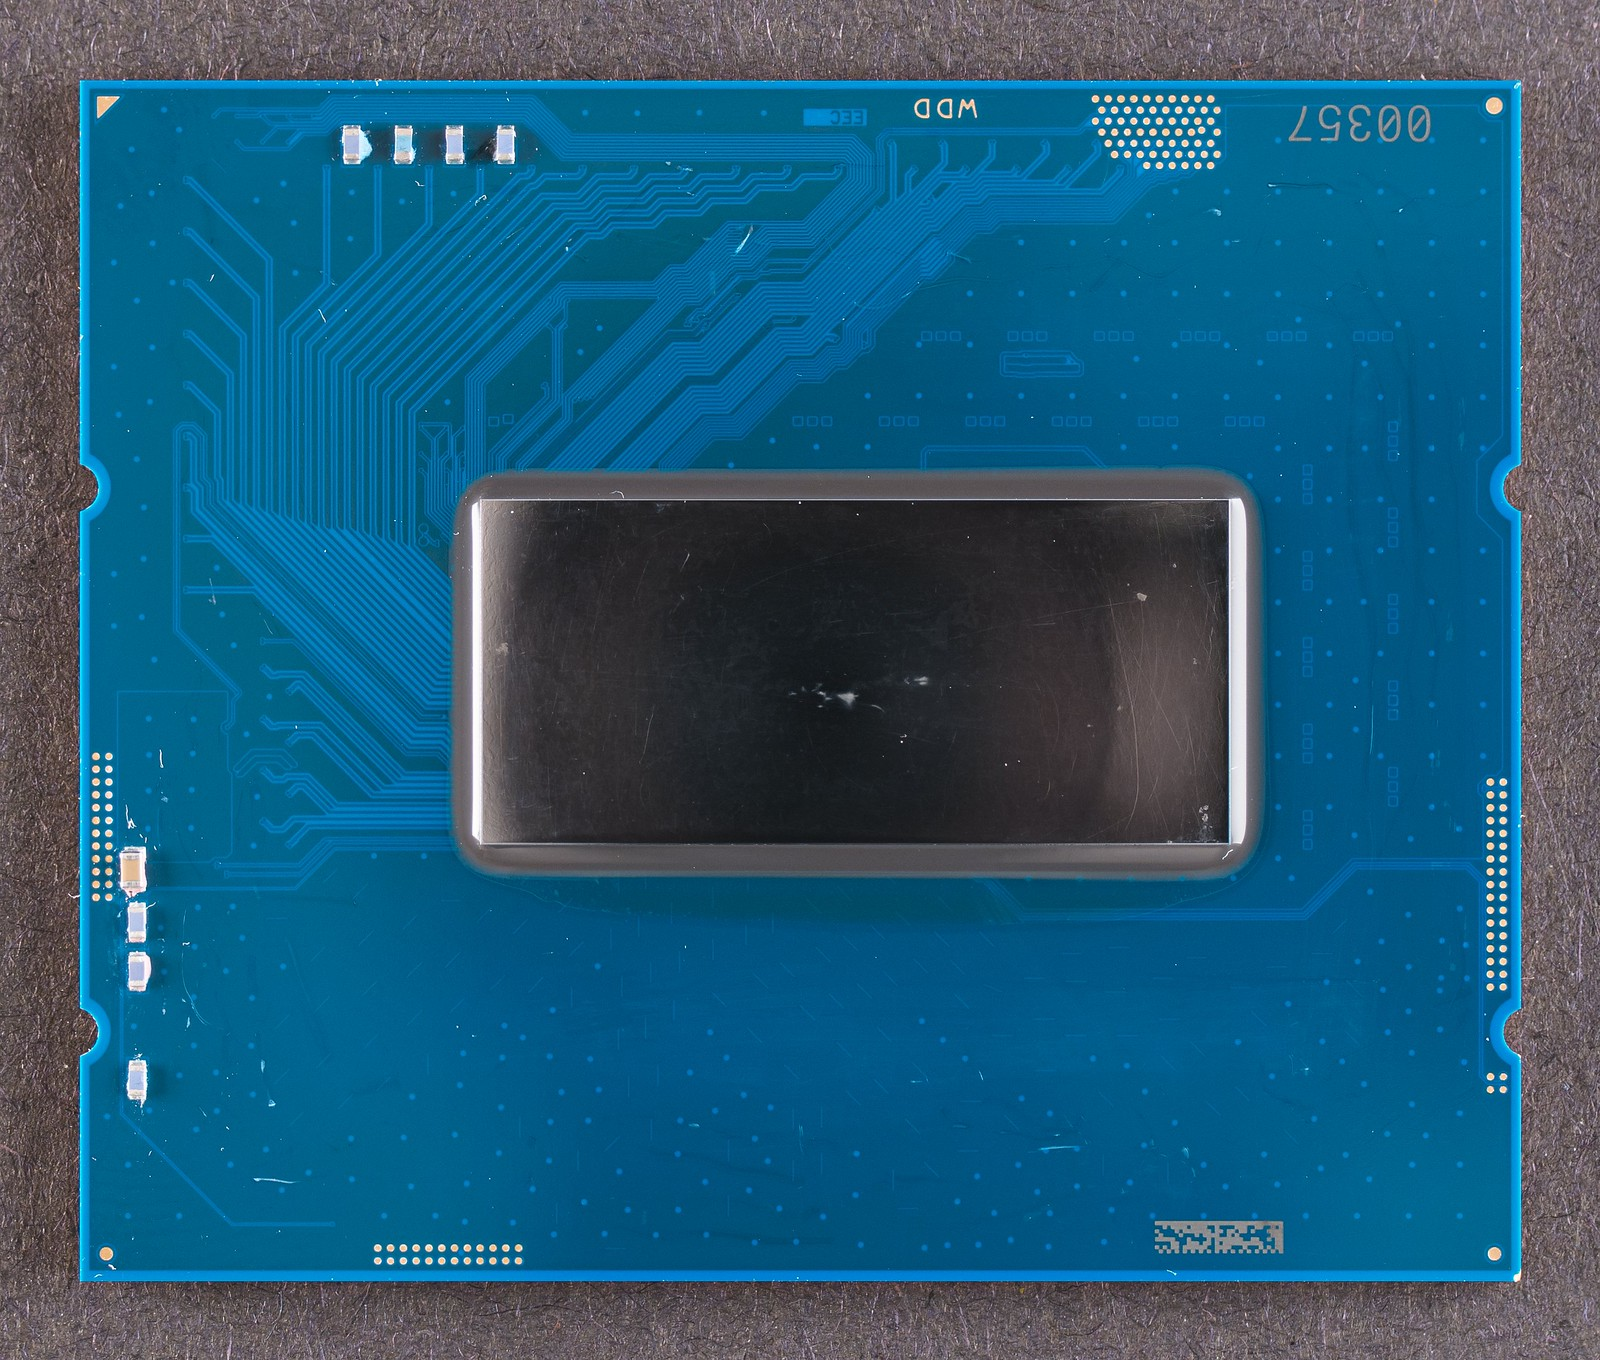
\includegraphics[width=0.44\linewidth]{silicon_chip.jpg}
  \hspace{0.2cm}
  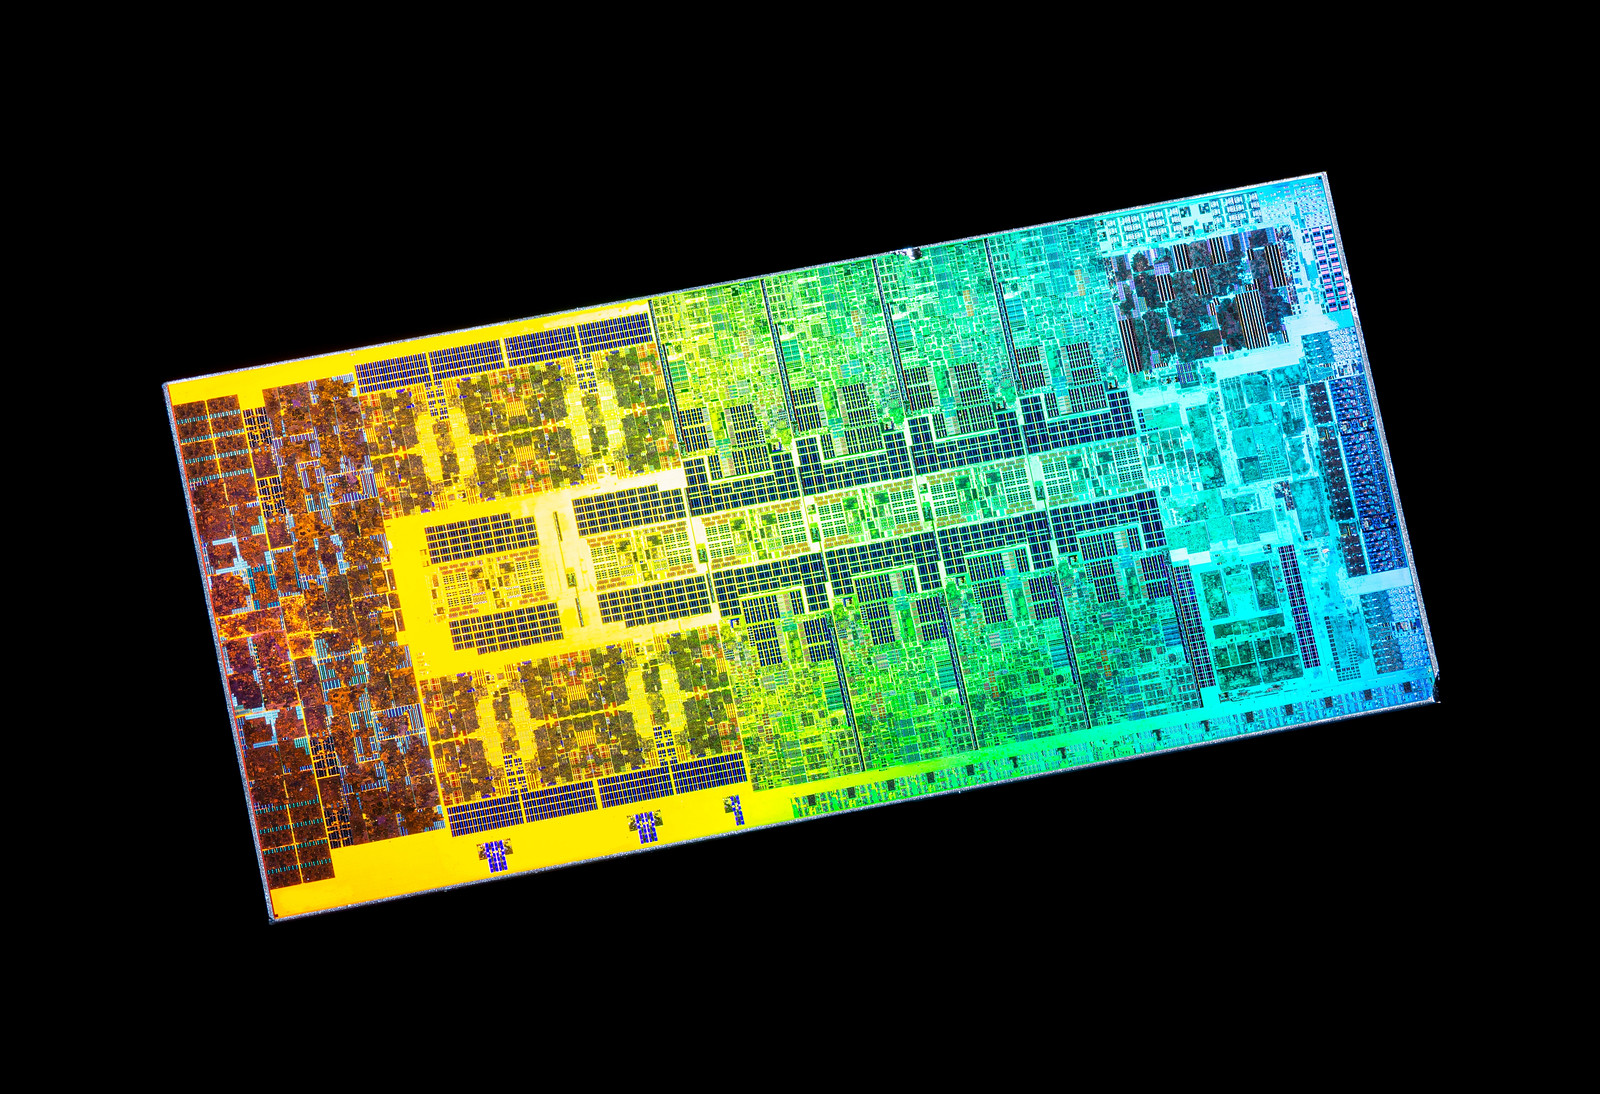
\includegraphics[width=0.36\linewidth]{silicon_die.jpg}
  \caption{封装后的芯片（左）和尚未封装的裸片（右）不是同一层次的对象。前者可上板装配，后者需要封装后才能进入产品。}
\end{figure}

先把这几个层次分开就好，不必一次性全记住。接下来两节会分别展开封装和板级系统——一颗裸片怎样变成能上板的器件，一颗芯片在板子上又怎样和电源、时钟、存储一起构成能跑的系统。顺便养成一个习惯：以后面对任何讨论，先问"在谈哪一层"，再问"这一层最关心什么"——很多争论的根源不是知识不够，是双方站在不同层次上说话。

\section{封装为什么必不可少}

\subsection{裸片不能直接进入产品}

裸片承载了真正的电路，但它并不是为直接使用而生的。片上焊盘的尺度通常在几十微米量级——比头发丝还细——没有任何常规焊接设备能直接把它们可靠地连到板级走线上。裸片本身也脆弱：轻碰就可能碎裂，暴露在空气中会受潮、氧化，静电也可能直接击穿它。

所以裸片往往需要经过封装，才能变成一颗可以运输、测试、焊接、装配、散热和维护的器件。从工程角度看，封装至少在做这几件事：

\begin{itemize}
  \item \textbf{机械保护}：为脆弱的硅片提供物理防护。
  \item \textbf{电连接引出}：把片上微米级焊盘转换成板级可焊接的引脚或焊球。
  \item \textbf{散热}：提供从裸片到散热器再到空气的热通路。
  \item \textbf{可测试性}：让器件能进入自动测试设备做筛选与量产测试。
  \item \textbf{可装配性}：让芯片能进入标准 SMT 产线自动装配。
\end{itemize}

\begin{warnbox}
封装不只是芯片做好之后顺手``套个壳''。从某种意义上说，没有封装就没有可用的芯片产品。
\end{warnbox}

\subsection{各式各样的封装}

DIP、SO、QFP、QFN、BGA 这些封装，不只是壳子的``样子不同''。每一种背后都有一组现实的工程权衡：引脚够不够多、面积能不能接受、热怎么散、信号路径会不会太长、装配成本高不高、坏了好不好修。

\begin{figure}[h]
  \centering
  \begin{tabular}{ccccc}
  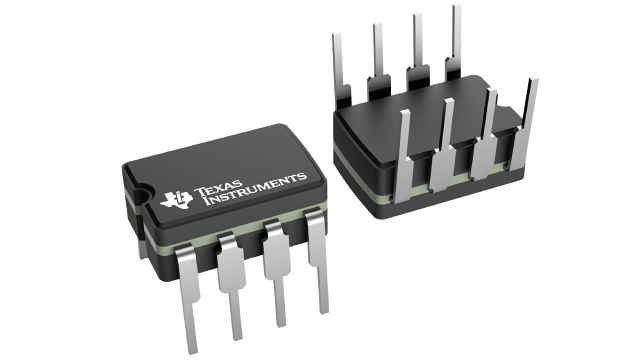
\includegraphics[width=0.16\linewidth]{DIP.png} &
  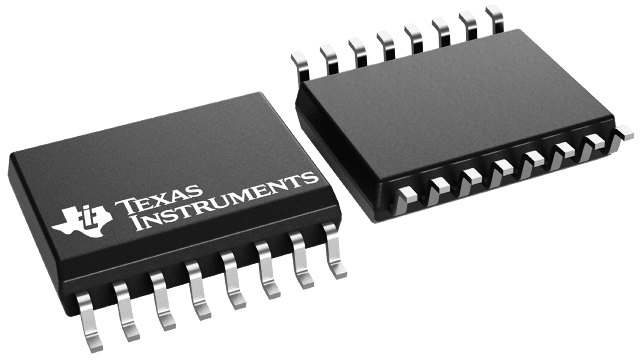
\includegraphics[width=0.16\linewidth]{SO.png} &
  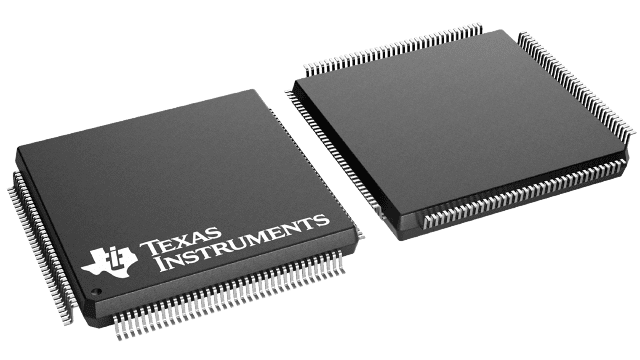
\includegraphics[width=0.16\linewidth]{QFP.png} &
  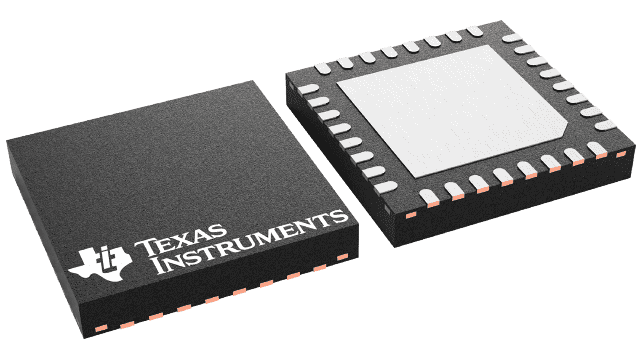
\includegraphics[width=0.16\linewidth]{QFN.png} &
  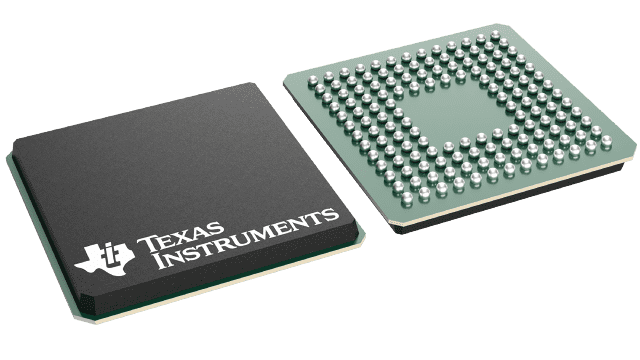
\includegraphics[width=0.16\linewidth]{BGA.png} \\
  \scriptsize DIP &
  \scriptsize SO &
  \scriptsize QFP &
  \scriptsize QFN &
  \scriptsize BGA
  \end{tabular}
  \caption{几种常见封装形式。它们不是单纯的外观变化，而是引脚密度、散热能力、信号完整性和装配成本的工程折中。}
\end{figure}

引脚少、速度低的芯片，封装可以做得简单，手工焊接也没问题；高性能芯片则几乎必然走向 BGA 甚至更复杂的封装形式。这里没有哪种``更好''的绝对答案——每种封装都是面积、成本、性能、散热和装配之间的一组具体折中。

\section{芯片在 PCB 系统中如何工作}

\subsection{芯片从来不是孤立工作的}

很多教材里的数字电路例子，会把芯片画成一个自给自足的逻辑盒子——给输入，内部自动计算，吐出输出。这种简化在入门时很有必要，但它也带来一个副作用：让人误以为芯片可以独立工作。但是在真实世界中，一颗芯片要真正跑起来，至少需要被放进一个板级环境里，和电源、时钟、复位、存储、外设一起构成闭环。

不妨看看最简单的 STM32 最小系统板。板上除了 MCU 芯片本身，还有晶振提供时钟、复位电路、3.3V 稳压电源、去耦电容，以及引出的 GPIO 和通信接口。如果你把 MCU 从板上拆下来单独供电——没有时钟源、没有复位电路、没有去耦电容——它不会工作。不是因为 MCU 坏了，而是因为它从来就不是为``孤独运行''设计的。

\begin{figure}[h]
  \centering
  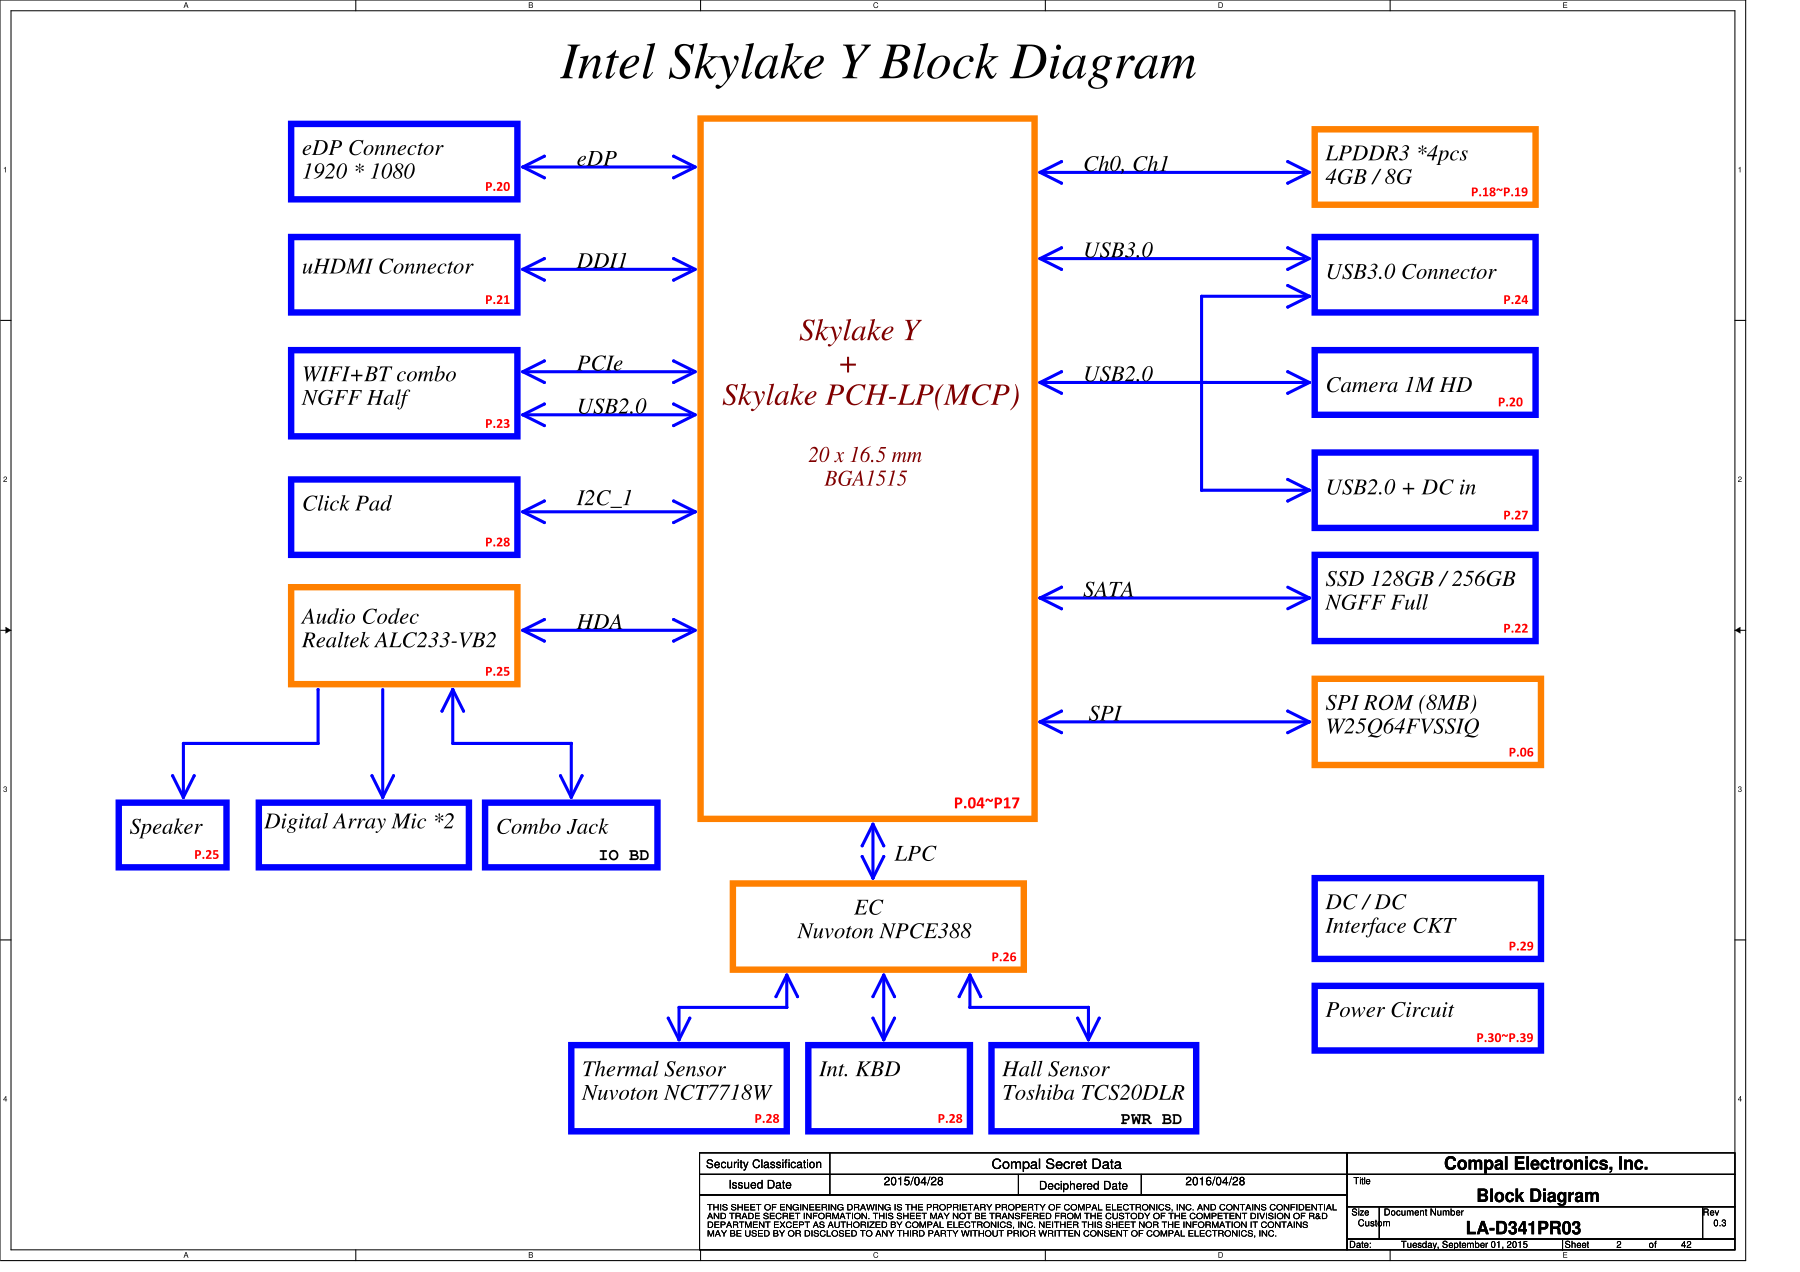
\includegraphics[width=1.0\linewidth]{system-block-diagram.png}
  \caption{一个笔记本主板的系统框图。CPU 不是唯一主角，它依赖电源、时钟、复位、存储和外设协同工作。}
\end{figure}

框图是抽象的，真实主板长这样。下面这张图是一块笔记本主板（MacBook Air M2），彩色框标出了主控芯片、存储器和电源管理器件的分布。即便不看具体型号，也能辨认出系统里各类角色的大致位置——这和框图里画的是同一套逻辑。

\begin{figure}[h]
  \centering
  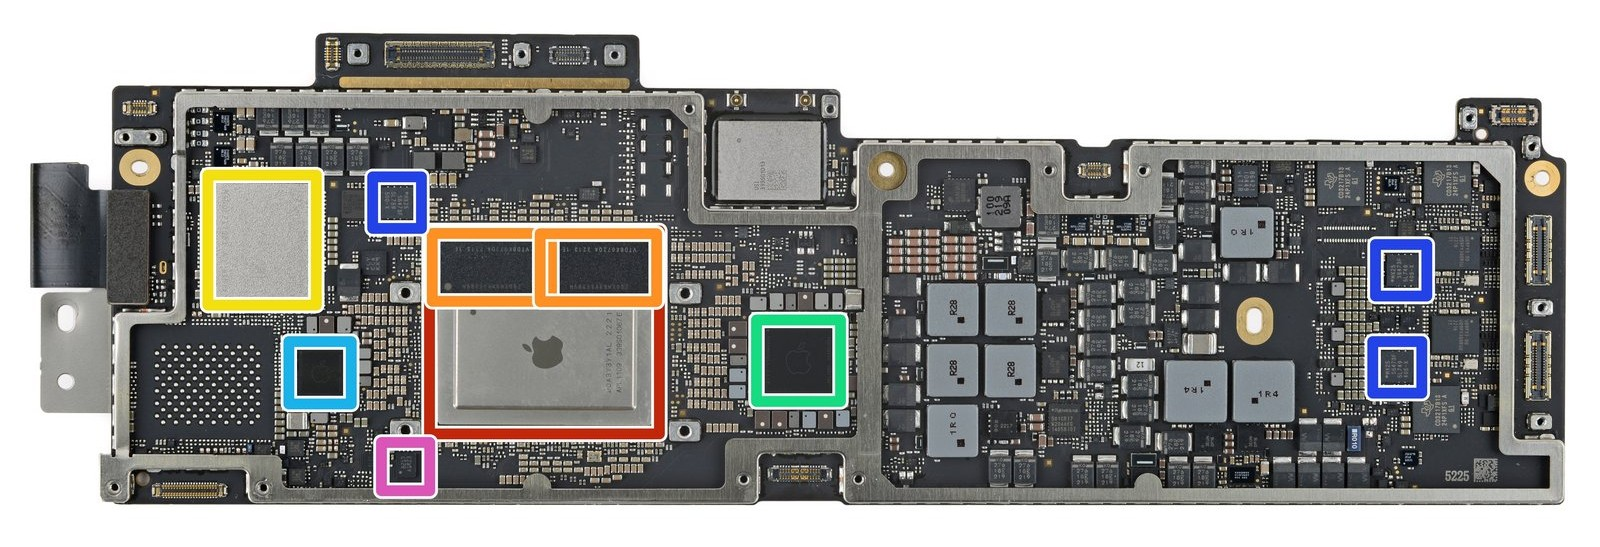
\includegraphics[width=1.0\linewidth]{mba_m2_motherboard.jpg}
  \caption{一块真实笔记本主板的俯视图。彩色框示意了不同功能模块的物理分布，与系统框图中的角色一一对应。}
\end{figure}

\subsection{理解一个板级系统的五个问题}

面对一块陌生的板卡，不妨先问自己下面五个问题。它们几乎适用于所有数字系统——从简单的 Arduino 开发板，到手机主板、SSD 控制板、路由器，甚至工业控制板：

\begin{enumerate}
  \item 主控芯片是谁，它负责计算、控制还是连接？
  \item 电源从哪里来，系统里有几个主要电压域？
  \item 时钟由谁提供，复位如何建立系统初态？
  \item 片外存储有哪些，它们与主芯片之间的关系是什么？
  \item 系统需要对外连接哪些接口或外设？
\end{enumerate}

这五个问题看起来很朴素，但它们有一个很强的好处：会强迫你把注意力从``芯片型号表演''拉回``系统关系''。你不需要一上来就知道每个芯片的型号和参数，也能先把系统的大骨架看出来。对于自学者来说，这比一开始猛背型号有效得多。

\subsection{电源、时钟、复位、存储与接口}

电源是芯片赖以工作的基础。现代芯片往往有多个电压域：核心逻辑、电平接口、模拟部分、存储器接口，它们常常使用不同的电源轨。电源不稳定会直接影响时序可靠性，因此去耦电容、PMIC 和供电网络是系统可靠性的基石，不是附属零件。你后面学到的时序问题，看起来像在讨论逻辑路径，很多时候也会被电源质量悄悄影响。

时钟是数字系统的``心跳''。寄存器在哪个边沿采样、状态机何时跳转、数据在哪个周期被传输，都以时钟为基准。在板级层面，时钟通常由外部晶振或振荡器提供，再由芯片内部 PLL 产生更高频率的工作时钟。后面学到的时钟树、时钟偏斜和时钟域，本质上都在服务同一个目标：维持系统节奏。

复位负责把系统带入可控起点。系统刚上电时，寄存器状态可能是不确定的；如果不加干预，处理器可能从随机地址开始取指，状态机可能跳进非法状态。复位的任务，就是等电源和时钟稳定后，把关键状态拉回预定义初值。这里也埋下一个后续会反复出现的判断：并非所有寄存器都需要同样严格的复位策略。

存储和接口把芯片放回真实系统中。主控芯片内部的 SRAM 容量有限，很多系统会依赖片外 Flash 和 DRAM。芯片也总要通过 USB、PCIe、DDR、I2C、SPI、UART、显示接口或传感器接口与外部世界协作。于是，``芯片设计''很少只是盯着一颗芯片本身，而更像是在理解它如何和周围对象配合工作。

这一节先学会看``骨架''就够了。至于每条接口具体怎么时序握手、每种存储器为什么这样组织、复位策略为什么还分同步和异步，这些后面都会一层层回来。

\begin{tipbox}
电源轨（Power Rail）可以理解为芯片内部的供电``专线''。不同功能模块往往对应不同的电源轨，它们在电压等级、电流能力、噪声容限和工作条件上各不相同。例如，CPU 核心可能运行在 0.8V 的低电压轨上以节省功耗，而 I/O 接口可能需要 3.3V 的电压轨来兼容外部设备。更精细的设计中，同一颗芯片的不同电源轨还可以独立开关——比如系统进入睡眠模式时，可以关闭 CPU 核心的供电轨，但保持实时时钟（RTC）的供电轨继续工作，从而在省电的同时不丢失时间信息。
\end{tipbox}

\section{常见芯片类型与系统角色}

\subsection{按角色的分类框架}

芯片类型很多，按市场产品名去记很快就会陷入混乱；更自然的办法，是按它在系统里承担什么``角色''来理解。下面不是一份芯片``名录''，而是一组按角色划分的梳理。每类都回答同一个问题：它在系统里干什么？

\begin{figure}[h]
  \centering
  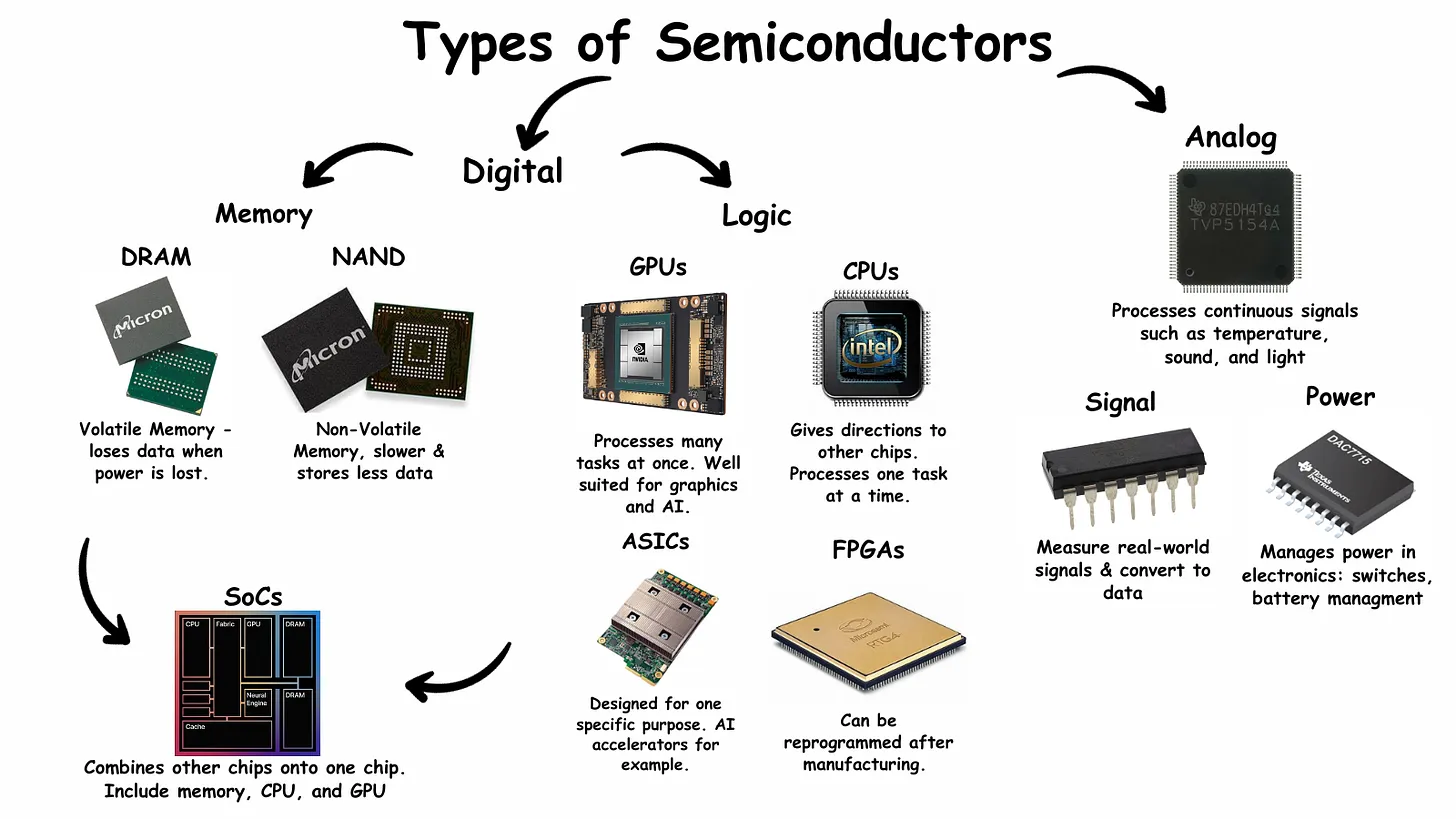
\includegraphics[width=0.94\linewidth]{type_of_chip.png}
  \caption{芯片类型地图。关键不在于背出名称，而在于理解每类芯片在系统中的功能位置。}
\end{figure}

\paragraph{计算类芯片}
CPU、GPU、DSP、AI 加速器——它们的核心任务都是计算，但面向的场景不同。CPU 像一位全能管家，擅长处理分支多、依赖复杂的程序逻辑；GPU 像一支整齐划一的军队，把几千个简单计算单元组织在一起，同时对大量数据做同一种操作；DSP 像一位音频工程师，针对 FFT、滤波、卷积这类信号处理算法做了专门的硬件优化；AI 加速器则像一台专用机床，专门为矩阵乘法和卷积操作设计硬件结构，通常作为 CPU/GPU 的协处理器出现。

\paragraph{控制类芯片}
MCU 和控制类 SoC 通常扮演系统主控的角色。它们不追求极端算力，但在外设控制、实时响应、功耗和成本上往往有严格的要求。STM32、ESP32、AVR 系列都属于这一类。一辆现代汽车里可能有几十甚至上百个 MCU，分别负责发动机控制、车窗升降、气囊触发、胎压监测——每个都是一个独立的小系统。

\paragraph{存储类芯片}
SRAM、DRAM、Flash 提供不同层次的容量、速度和掉电保持特性。设计一个数字系统，不只是``算得快''的问题，还包括``数据放在哪里、何时搬运、掉电后还在不在''——存储是计算的搭档，不是附属品。

\paragraph{可编程类芯片}
FPGA 是一种特殊的芯片：它的硬件逻辑在出厂后仍可被重新配置。这让它在教学（一块板子可以反复变成不同电路）、原型验证（流片前用 FPGA 高速模拟设计行为）以及小批量灵活性场景中都很有价值。

\paragraph{接口、模拟与电源类芯片}
一个系统很少只靠一颗主控芯片跑完全程。PHY 芯片负责把数字信号变成适合特定介质传输的物理波形；桥接芯片在不同总线协议之间做翻译（比如 PCIe 转 SATA、USB 转 UART）；PMIC 为系统提供多路稳定供电；ADC / DAC 在模拟世界和数字世界之间守门；PLL 生成精确时钟；温度传感器、加速度计、光学传感器等则让系统感知外部环境。这些器件不一定是系统里最显眼的``主角''，但它们常常是决定系统能否稳定工作的关键支撑。

\begin{tipbox}
下次拆开一个电子产品时，不妨先按角色归位：哪些是计算/控制的？哪些是存储的？哪些是接口/电源/模拟的？先建立角色感，再去看具体型号——角色比型号更稳定，也更容易记住。
\end{tipbox}

\section{从想法到产品：设计流程与产业链}

\subsection{设计流程为什么重要}

一颗数字芯片从需求想法走到最终制造，不是``写完代码就结束''的事情。它是一条跨学科、跨岗位、跨工具链的长链路。设计流程之所以重要，不是因为术语多，而是因为每一步都在交付不同层次的结果，也都在把上一步的抽象继续往现实推进。

\begin{figure}[h]
  \centering
  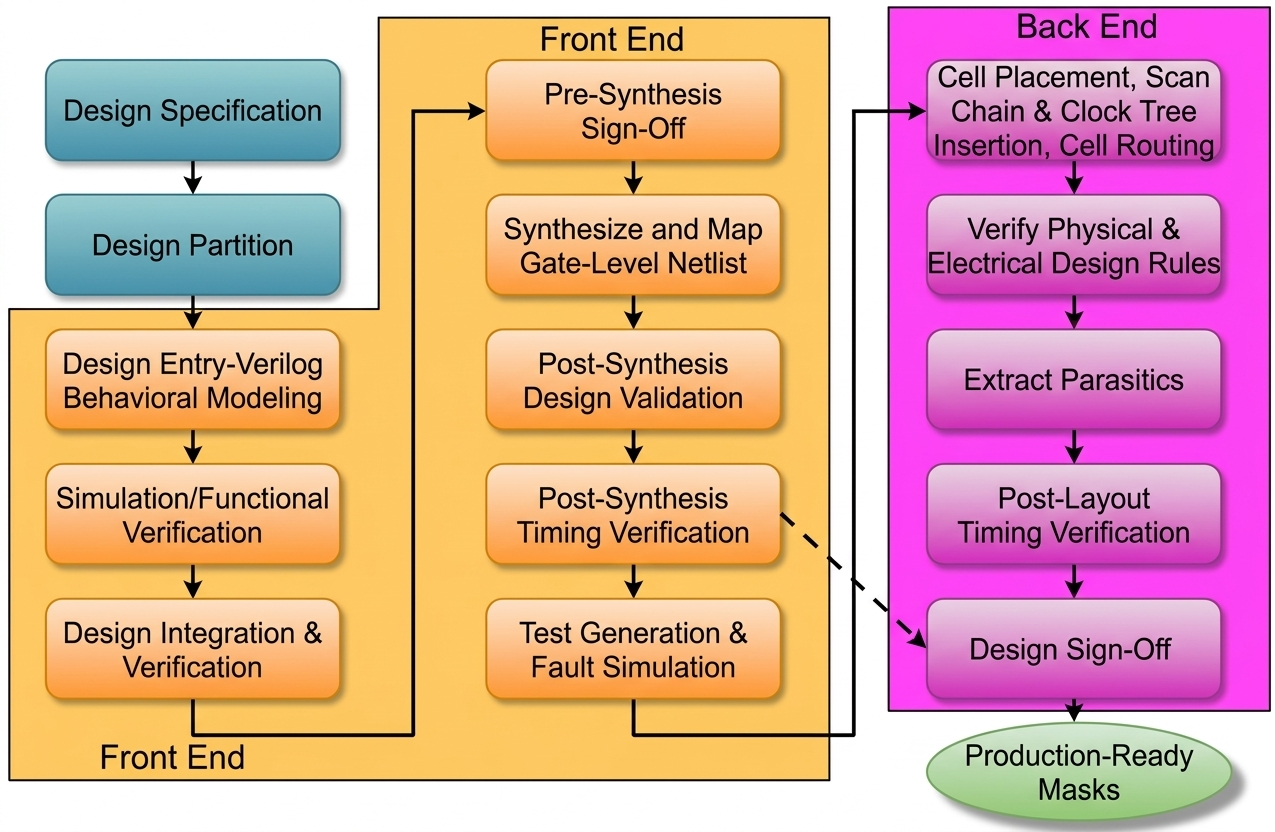
\includegraphics[width=0.8\linewidth]{digital_flow.jpeg}
  \caption{一个简化的数字芯片设计流程示意。每个阶段消费上一层的结果，交付下一层的输入。}
\end{figure}

以一个简化的数字芯片项目为例：产品需求先给出功能、功耗和成本目标；架构阶段把目标拆成可实现的子系统；RTL 阶段用 HDL 描述寄存器与组合逻辑行为；验证阶段确认 RTL 是否满足规格；综合阶段把 RTL 映射成门级网表；物理实现阶段完成布局布线、时钟树和寄生处理；最后通过签核并交付流片。越早阶段犯下的错误，修复代价往往越大。

你可以把这个过程想象成盖房子。需求和架构像是在定用途和画总图；RTL 像是在把结构和空间划分真正画出来；验证像是在确认这张图没有自相矛盾；综合和物理实现则开始受到材料、尺寸、承重和施工工艺的真实约束。图纸阶段改一堵墙和楼已经封顶后再改一堵墙，代价当然不会一样。芯片设计也是同理。

\subsection{几个核心阶段的简介}

\begin{enumerate}
  \item \textbf{需求定义与架构设计}：回答``要做什么''和``怎么组织''，产出功能规格书、模块划分图和接口定义。
  \item \textbf{RTL 设计}：用可综合 HDL 描述寄存器与组合逻辑行为。这是后续课程会花大量时间进入的核心工作面。
  \item \textbf{功能验证}：确认 RTL 是否真正满足规格要求。现代芯片项目中，验证常常消耗极大比例的总工时。
  \item \textbf{逻辑综合}：把 RTL 映射成目标工艺库上的门级网表，并结合时钟、输入输出延迟等约束进行优化。
  \item \textbf{物理实现}：完成布局布线、时钟树综合、电源网络和时序签核，把功能描述变成真实几何结构。
  \item \textbf{签核与流片}：在功能、电气、时序和物理规则都满足要求后，交付版图数据给晶圆厂制造。
\end{enumerate}

设计流程的价值在于：你能看清后面每一章在整条链路上处于什么位置。学 RTL 时，你处在架构与实现之间；学综合时，你在把行为描述压成门级结构；学时序与物理实现时，你也在继续把抽象一层层落到现实。对自学者而言，这种位置感尤其重要——一旦知道一个主题属于流程的哪一段，阅读时就更容易分清``这是主线''、``这是支线''、``这是后面还会回来的问题''。

从学习体验上说，这种``位置感''会明显减轻焦虑。因为很多术语并不是难在它本身，而是难在你不知道它为什么突然出现。只要知道一个概念属于流程的哪一段、解决哪一类问题，理解它就会容易很多。

\begin{warnbox}
不要误以为流程是线性的。在实践中，各个阶段之间会有大量迭代。综合发现时序违规可能需要回到 RTL 修改微架构；布局布线发现拥塞也可能迫使重新划分模块边界。
\end{warnbox}

\subsection{产业链角色与代表公司}

很多人一开始会把所有和半导体有关的公司都叫``芯片公司''。这个说法不算错，但太粗了——粗到会掩盖产业结构中最关键的分工。事实上，半导体产业链高度专业化：有的公司卖 IP，有的卖 EDA 工具，有的负责芯片设计和产品定义，有的专做晶圆制造，有的做封装测试，还有的提供设备和材料。把 ARM、Synopsys、NVIDIA、TSMC、ASE、ASML 都叫``芯片公司''，有点像把建筑师、CAD 软件公司、房地产开发商、施工队、监理和水泥厂都叫``盖房子的''——技术上没错，但完全模糊了它们各自的业务模式和风险结构。

\begin{figure}[h]
  \centering
  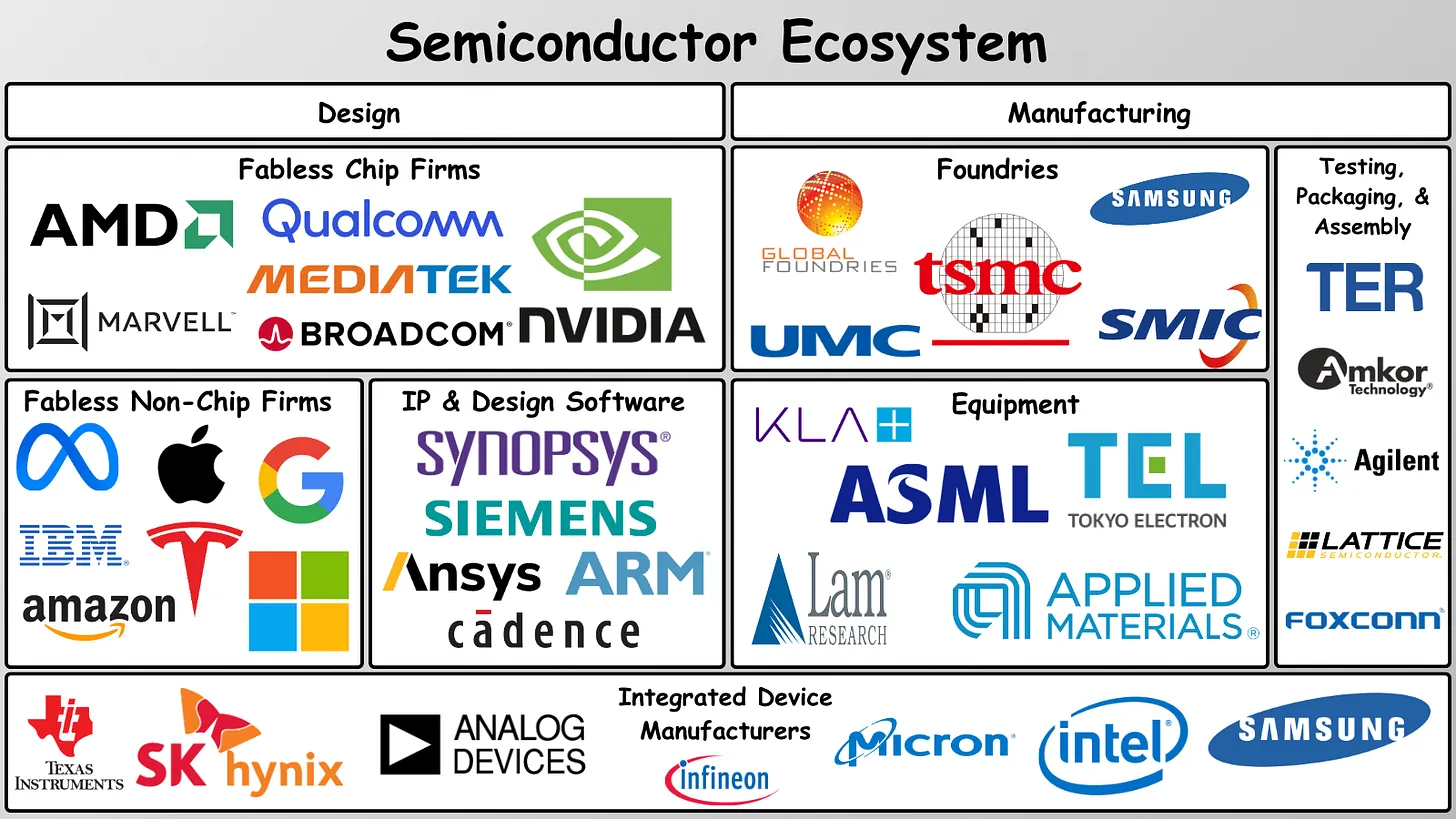
\includegraphics[width=0.96\linewidth]{semi_ecosys.png}
  \caption{半导体生态系统示意。不同类别公司在输入、输出和责任边界上显著不同。}
  \label{fig:semi_ecosys}
\end{figure}

\paragraph{IP 公司}
IP 公司提供可复用的设计模块，例如 CPU 核、GPU 核、USB / PCIe / DDR PHY、总线组件和存储控制器。ARM、Imagination 等公司都属于这一类。它们的价值在于把高复杂度功能做成可授权、可集成的标准化模块。

\paragraph{EDA 公司}
EDA 公司提供设计、验证、综合、实现、签核和分析工具。Synopsys、Cadence、Siemens EDA 是这一领域的代表。没有这些工具，现代大规模芯片几乎无法工程化落地。

\paragraph{Fabless / Design House}
这类公司负责芯片定义、架构、RTL 设计、验证、物理实现和产品化，但通常不拥有自己的先进晶圆制造厂。NVIDIA、AMD、Qualcomm、Broadcom、MediaTek、海思、紫光展锐等都属于这一类。它们的核心能力在于产品定义和设计能力。

\paragraph{Foundry}
晶圆厂负责把设计转换为真实硅片。TSMC、Samsung Foundry、GlobalFoundries、SMIC 等都属于 Foundry。它们的核心能力在工艺制程、良率控制、大规模生产和设备运营。

\paragraph{OSAT}
OSAT 连接了晶圆制造和最终器件交付，负责晶圆切割、芯片封装和最终测试。ASE、Amkor、长电科技等是这一领域的代表。先进封装在很多场景下已经成为高性能芯片的重要使能技术。

\paragraph{设备与材料公司}
没有光刻机、刻蚀机、沉积设备、检测设备以及高纯度硅片、光刻胶和特种气体，制造环节本身无法存在。ASML、Applied Materials、Lam Research、Tokyo Electron 等公司构成了这条链路的物理基础。

这类常识看起来有点``行业八卦''，其实非常实用。因为一旦你知道一家公司在链条上的位置，你就更容易判断它为什么强调某些能力、为什么会发布某些产品、为什么它的新闻里总在谈工艺、生态、IP 授权或者工具链，而不是别的东西。

\begin{tipbox}
一个小练习：找出你熟悉的电子产品里至少 3 颗主要芯片，尝试回答它们是谁设计的、谁制造的、谁封装的，背后可能用了哪些 IP 和 EDA 工具。不一定全对，但这个过程会让你对产业链有真实的体感。
\end{tipbox}

\subsection{生态、工具与服务}

产业链分析回答了``谁在做什么''，但真实世界的竞争并不只发生在硅片制造这一层。工具链、文档、参考设计、技术支持和开发者生态，常常也会显著改变一家公司在市场上的竞争力。

台积电不只是``代工制造''，还提供 PDK、设计规则、技术支持和工艺协同优化；ARM 不只是``卖 IP 核''，还提供工具、参考设计、培训和生态支持；很多设计公司向下游客户交付的也不只是芯片本体，更包括配套文档、开发工具、参考设计和 FAE 支持。芯片行业首先是一个高度分工的技术产业，但它并不只是``把硅片做出来''这么简单。

如果把这件事说得再贴近一点：很多学生第一次真正``感受''一个芯片公司好不好，与其说是在看晶体管数量，不如说是在下载文档、找例程、配环境、查论坛、问问题的时候。好用不好用、顺手不顺手，往往就是在这些环节被体会到的。工程世界里，产品本体当然重要，但围绕产品建立的可用性也同样重要。

一些直观的具体案例可以让我们清楚感受到这一点：STM32 之所以成为大量教学和工程项目的入口，不只是因为芯片参数合适符合用户需要，还因为 HAL / LL 库、开发板、文档、社区和参考设计足够完整——用起来顺手，选它的概率就高；CUDA 之所以形成强大壁垒，也不只是因为 GPU 硬件性能，还因为围绕它形成了完整的软件栈、工具链和开发者生态。重点不是把这些案例神化，而是意识到：芯片竞争经常发生在``芯片之外''。

对很多同学来说，第一次真正接触``芯片行业''并不是进公司实习，而是在做开发板、小系统和实验项目时，开始和芯片公司的文档、论坛、例程、参考设计以及社区讨论打交道。等你以后真的参与到板级小系统开发时，也可以试着去体会这种来自社区和技术支持体系的帮助：多查资料，多问问题，多看别人是怎么定位和解决问题的。TI、Xilinx、ADI、STMicroelectronics、Infineon、OnSemi 等公司的资料、论坛和工具，常常会让人第一次具体地感受到芯片行业每天到底在``发生什么''。在这个过程里，很多知识不只来自课本，更是在和文档、社区、开发板、例程的来回碰撞中慢慢长出来的。

这几年，中文世界和本土社区的支持也在明显变强。像沁恒微、Espressif、Nuvoton 等公司，以及 Sipeed 这样的开发板供应方，都在文档、工具、论坛、开源例程和社区传播上提供了很大的帮助。对学习者而言，这些支持是真实而具体的；对整个开源硬件社区来说，它们也在持续降低入门门槛、扩大参与者的数量。

开放资料在 AI / LLM 时代还获得了另一层价值。结构化、可公开获取的文档、应用笔记和参考设计，会更容易进入开发者的检索链路，也更容易被新一代工具学习和引用。这不意味着``开放''可以取代产品本身，但它确实会改变品牌触达和生态扩散的速度。

\section{设计准则与 3Y 三问法}

\subsection{全书的工程准则}

最后一节只做一件事：收束几条在全书都会反复出现的工程准则。它们不是额外的知识点，而是你看待设计问题的默认视角：

\begin{itemize}
  \item \textbf{抽象优先}：面对任何设计问题，先确定讨论在哪个抽象层上，再谈具体方案。
  \item \textbf{模块化}：把系统切成可验证、可替换、可复用的模块。
  \item \textbf{接口清晰}：输入输出、时序、数据格式和约束条件要尽量明确。
  \item \textbf{尽早验证}：问题越晚暴露，修复代价越高。
  \item \textbf{用约束管理复杂度}：面积、性能、功耗、时序不是设计完成后才考虑的附属品，而是与功能同等重要的输入。
\end{itemize}

\subsection{3Y 三问法}

为了避免只停留在``知道一个功能名字''的模糊理解上，我们在整个学习过程中会反复使用一个简单的思考框架：3Y 三问法。面对任何芯片、模块或子系统，先问自己三个问题：

\begin{itemize}
  \item \textbf{Why}：为什么要做它？它解决什么问题？目标和约束是什么？
  \item \textbf{What}：它到底是什么？功能边界在哪里？输入是什么，输出是什么？
  \item \textbf{How}：它如何实现？用怎样的结构、时序组织和状态管理来保证它可实现、可验证、可维护？
\end{itemize}

这三个问题并不神秘，但可以把一个模糊印象拆成三个可独立回答的方向。Why 定义目标，What 定义边界，How 定义实现。后面无论遇到加法器、状态机、FIFO、流水线处理器还是整个 SoC，都可以先用 3Y 过一遍。

\begin{tipbox}
3Y 不是让你跳过技术细节，而是帮你在钻进细节之前，先把问题的轮廓画清楚。
\end{tipbox}

\section{本章小结}

让我们回顾一下这一章走过的路：

\begin{itemize}
  \item 数字系统依赖抽象与分层，不是因为这样``高级''——复杂度已经大到很难从器件层直接穷举设计。
  \item 数字抽象把连续的物理世界组织成离散的逻辑世界，但它依赖电平、时序和接口边界这些工程前提——前提一旦被打破，抽象就会崩塌。
  \item 从分立电路到 IC 再到 SoC，集成化已经成为现代电子系统的主导范式，而且这种趋势同时发生在数字、模拟和混合信号领域。
  \item 裸片（die）通常要经过封装（package），才能成为可上板、可装配、可散热、可测试的器件（chip）。
  \item 芯片不是孤立发光的小黑块，而是系统中的一个角色——它依赖电源、时钟、复位、存储和接口才能工作。
  \item 芯片世界不是一家公司从头到尾的直线流程，而是高度分工的产业链：IP、EDA、Fabless、Foundry、OSAT、设备与材料各司其职。
  \item 产业链的主线是角色分工，但工具、文档、生态和支持体系也会显著影响芯片公司的竞争力。
  \item 面对任何设计和学习对象，3Y（Why / What / How）都是一个先把问题站稳的实用习惯。
\end{itemize}

这些判断不需要你一次性全背下来。更合理的做法是：在读后面章节时，每当遇到新概念，试着把它放回这张地图里，问自己``它在哪个抽象层？它在系统里扮演什么角色？它在设计流程的哪一段？''久而久之，这个图景会从纸上的文字变成你脑子里的一套直觉。

第二章开始，我们就会顺着这个框架往下走，进入工具、环境和最小实践闭环。那时你大概会发现：前面这一章看上去像是在``绕远路''，其实是在给后面的每一步省力。因为只要框架在手，后面的概念就不再是孤零零地出现，而是会自动落回它原本应该在的位置。

\section{术语表}

\begin{center}
\begin{tabular}{p{0.22\linewidth} p{0.68\linewidth}}
\toprule
术语 & 简要说明 \\
\midrule
\texttt{die} & 尚未封装的裸片，承载晶体管和互连的硅本体。 \\
\texttt{package} & 为裸片提供保护、电连接、散热和装配形态的封装结构。 \\
\texttt{chip} & 日常工程语境中通常指封装完成后的芯片器件。 \\
\texttt{PCB} & Printed Circuit Board，印刷电路板。 \\
\texttt{SoC} & System on Chip，在单芯片上集成多个功能模块的系统级芯片。 \\
\texttt{RTL} & Register Transfer Level，寄存器传输级设计抽象。 \\
\texttt{EDA} & Electronic Design Automation，电子设计自动化工具链。 \\
\texttt{Fabless} & 无晶圆制造厂、主要负责设计与产品定义的公司模式。 \\
\texttt{Foundry} & 负责晶圆制造的代工厂。 \\
\texttt{OSAT} & Outsourced Semiconductor Assembly and Test，外包封装测试。 \\
\texttt{PMIC} & Power Management IC，电源管理集成电路。 \\
\texttt{PLL} & Phase-Locked Loop，锁相环，用于时钟生成和倍频。 \\
\texttt{IP核} & Intellectual Property Core，可复用的设计模块（如 CPU 核、接口控制器）。 \\
\texttt{Moore's Law} & 摩尔定律：集成电路上晶体管数量约每两年翻一番的经验性观察。 \\
\texttt{IC} & Integrated Circuit，集成电路。 \\
\texttt{Op-Amp} & Operational Amplifier，运算放大器。 \\
\texttt{PDK} & Process Design Kit，工艺设计套件。 \\
\texttt{FAE} & Field Application Engineer，现场应用工程师。 \\
\texttt{LLM} & Large Language Model，大型语言模型。 \\
\bottomrule
\end{tabular}
\end{center}

\section{练习题}

\begin{enumerate}
  \item 试着用自己的话解释 \texttt{die}、\texttt{package}、\texttt{chip}、\texttt{board} 和 \texttt{system} 之间的关系。如果有人说我电脑里的``芯片''坏了，他说的可能是哪个层次的对象？
  \item 集成电路从真空管走到晶体管，再走到 IC，中间经历了哪些关键转折？Kilby 和 Noyce 各自贡献了什么？为什么 Noyce 的硅平面工艺最终成为主流？
  \item 为什么说集成化已经成为现代电子系统的主导范式？请至少从数字、模拟或混合信号中的两个角度举例说明。
  \item 比较分立电路方案和集成芯片方案在成本、体积、可靠性和开发效率上的差异。举出一个你身边的例子——比如手机充电器、蓝牙音响、或者你正在用的鼠标。
  \item 画一个最小板级系统框图，至少包含主控芯片、存储、电源模块、时钟源和一个外设接口，标注每个部分的作用和数据流向。
  \item 数字抽象为什么不是天然成立的？请结合电平、时序和接口边界三个方面作答，每个方面各举一个``抽象失效''的具体场景。
  \item 选一个你手边的电子产品（手机、路由器、开发板、SSD、智能手表、游戏机都可以），拆开它或者查资料，列出其中至少 4 颗芯片或关键器件，并说明它们各自在系统中承担什么角色。
  \item 画出一条简化的数字芯片设计流程，说明每一阶段主要交付什么。再试着解释：为什么越早阶段犯下的错误，修复代价越大？
  \item 在图~\ref{fig:semi_ecosys} 中选几类公司，查一查它们的代表企业，说说它们主要做什么、在产业链中处于什么位置。
  \item 找一家你熟悉的公司（比如手机里的芯片品牌、电脑里的处理器品牌），判断它更像是在卖 IP、卖 EDA、做 Fabless、做 Foundry、做 OSAT，还是做设备与材料。给出你的理由。
  \item 芯片行业的竞争为什么不只发生在制造环节？结合文档、开发工具、参考设计、技术支持或开发者生态中的任意两项，说说你的理解。
  \item 选一个你熟悉的模块或芯片（可以是手机里的某个功能，也可以是电脑上的某个接口），用 3Y 三问法写一段简要分析：Why、What、How 分别是什么。
\end{enumerate}

\end{document}
